%%%%%%%%%%%%%%%%%%%%%%%%%%%%%%%%%%%%%%%%%%%%%%%%%%%%%%%%%%%%%%%%%%%%%%%%%%%%%%%%%%%%%%%%% 
%%%%%%%%%%%%%%%%%%%%%%%%%%%%%%%%%%%%%% Preambule %%%%%%%%%%%%%%%%%%%%%%%%%%%%%%%%%%%%%%%%%
%%%%%%%%%%%%%%%%%%%%%%%%%%%%%%%%%%%%%%%%%%%%%%%%%%%%%%%%%%%%%%%%%%%%%%%%%%%%%%%%%%%%%%%%%%

\documentclass[a4paper, 12pt, leqno]{article}\usepackage[]{graphicx}\usepackage[]{color}
%% maxwidth is the original width if it is less than linewidth
%% otherwise use linewidth (to make sure the graphics do not exceed the margin)
\makeatletter
\def\maxwidth{ %
  \ifdim\Gin@nat@width>\linewidth
    \linewidth
  \else
    \Gin@nat@width
  \fi
}
\makeatother

\definecolor{fgcolor}{rgb}{0.345, 0.345, 0.345}
\newcommand{\hlnum}[1]{\textcolor[rgb]{0.686,0.059,0.569}{#1}}%
\newcommand{\hlstr}[1]{\textcolor[rgb]{0.192,0.494,0.8}{#1}}%
\newcommand{\hlcom}[1]{\textcolor[rgb]{0.678,0.584,0.686}{\textit{#1}}}%
\newcommand{\hlopt}[1]{\textcolor[rgb]{0,0,0}{#1}}%
\newcommand{\hlstd}[1]{\textcolor[rgb]{0.345,0.345,0.345}{#1}}%
\newcommand{\hlkwa}[1]{\textcolor[rgb]{0.161,0.373,0.58}{\textbf{#1}}}%
\newcommand{\hlkwb}[1]{\textcolor[rgb]{0.69,0.353,0.396}{#1}}%
\newcommand{\hlkwc}[1]{\textcolor[rgb]{0.333,0.667,0.333}{#1}}%
\newcommand{\hlkwd}[1]{\textcolor[rgb]{0.737,0.353,0.396}{\textbf{#1}}}%

\usepackage{framed}
\makeatletter
\newenvironment{kframe}{%
 \def\at@end@of@kframe{}%
 \ifinner\ifhmode%
  \def\at@end@of@kframe{\end{minipage}}%
  \begin{minipage}{\columnwidth}%
 \fi\fi%
 \def\FrameCommand##1{\hskip\@totalleftmargin \hskip-\fboxsep
 \colorbox{shadecolor}{##1}\hskip-\fboxsep
     % There is no \\@totalrightmargin, so:
     \hskip-\linewidth \hskip-\@totalleftmargin \hskip\columnwidth}%
 \MakeFramed {\advance\hsize-\width
   \@totalleftmargin\z@ \linewidth\hsize
   \@setminipage}}%
 {\par\unskip\endMakeFramed%
 \at@end@of@kframe}
\makeatother

\definecolor{shadecolor}{rgb}{.97, .97, .97}
\definecolor{messagecolor}{rgb}{0, 0, 0}
\definecolor{warningcolor}{rgb}{1, 0, 1}
\definecolor{errorcolor}{rgb}{1, 0, 0}
\newenvironment{knitrout}{}{} % an empty environment to be redefined in TeX

\usepackage{alltt} %leqno: numéro d'équation à gauche
\pagenumbering{arabic} % choose how to number the pages
\usepackage{a4wide}
%\usepackage[utf8]{inputenc} % accents interprétés
\usepackage{graphicx}
%\usepackage{subfig}
%\usepackage[hmargin=2cm, vmargin = 2cm, noheadfoot]{geometry} %% Pour gérer le format des pages
%\usepackage{layout} %% Pour avoir la longueur des marges
\usepackage[round,sort]{natbib} %% Natbib is a popular style for formatting references.
%\usepackage{multibib}
%\newcites{secnm}{Bibliographie} 
\usepackage{verbatim} % for multiline comments
\usepackage{amssymb} %symbole de maths
\usepackage{amsmath} %idem
%\usepackage{stmaryrd} %% Symbole flèche à l'envers
\usepackage{amsfonts}
\usepackage[english]{babel} %% Les titres en anglais
\usepackage[utf8]{inputenc} % accents interprétés
\usepackage{array} %% Pour centrer verticalement le contenu d'un tableau, entre autres...
\setcounter{secnumdepth}{4} %% Profondeur des sections, subsections
\usepackage{setspace} %% Gère l'interligne: singlespacing, doublespacing
\singlespacing
\usepackage[colorlinks=true,citecolor=blue]{hyperref} %% Gère les hyperliens
%\usepackage{textcomp} %% Symbole pourmille
\usepackage{lineno} %% Numérotation des lignes
\usepackage{lscape}
\usepackage{longtable}
\setlength{\LTleft}{-5cm plus 1 fill}
\setlength{\LTright}{-5cm plus 1 fill}
\usepackage{booktabs}
%\usepackage{colortabs} % can't be found
%\usepackage{xcolor}
%\usepackage{colortbl} %% color text and table rows
%\usepackage{arydshln} %% dashlines for tabular
%\usepackage{sidecap}
\newcommand{\logit}{\text{logit}}
\newcommand{\bs}[1]{\boldsymbol{#1}}
\newcommand{\p}{\text{p}}
% For changes in tables
\newcommand{\SetRowColor}[1]{\noalign{\gdef\RowColorName{#1}}\rowcolor{\RowColorName}}
\definecolor{gray90}{gray}{0.9}
\newcommand{\mymulticolumn}[3]{\multicolumn{#1}{>{\columncolor{gray90}}#2}{#3}}
\newcommand{\sizeBigTable}{\fontsize{9pt}{9pt}\selectfont}
\usepackage[section]{placeins} % Figures in section

\newcolumntype{L}[1]{>{\raggedright\let\newline\\\arraybackslash\hspace{0pt}}p{#1}}
\newcolumntype{C}[1]{>{\centering\let\newline\\\arraybackslash\hspace{0pt}}p{#1}}
\newcolumntype{R}[1]{>{\raggedleft\let\newline\\\arraybackslash\hspace{0pt}}p{#1}}

%%%%%%%%%%%%%%%%%%%%%%%%%%%%%%%%%%%%%%%%%%%%%%%%%%%%%%%%%%%%%%%%%%%%%%%%%%%%%%%%%%%%%%%%%%
%%%%%%%%%%%%%%%%%%%%%%%%%%%%%%%%%%%%%% Title %%%%%%%%%%%%%%%%%%%%%%%%%%%%%%%%%%%%%%%%%%%%%
%%%%%%%%%%%%%%%%%%%%%%%%%%%%%%%%%%%%%%%%%%%%%%%%%%%%%%%%%%%%%%%%%%%%%%%%%%%%%%%%%%%%%%%%%%

\title{Hierarchical Bayesian species distribution models with the \textbf{hSDM} R Package}
\date{\today}
\author{}

%%%%%%%%%%%%%%%%%%%%%%%%%%%%%%%%%%%%%%%%%%%%%%%%%%%%%%%%%%%%%%%%%%%%%%%%%%%%%%%%%%%%%%%%%%
%%%%%%%%%%%%%%%%%%%%%%%%%%%%%%%%%%%%%% Knitr %%%%%%%%%%%%%%%%%%%%%%%%%%%%%%%%%%%%%%%%%%%%%
%%%%%%%%%%%%%%%%%%%%%%%%%%%%%%%%%%%%%%%%%%%%%%%%%%%%%%%%%%%%%%%%%%%%%%%%%%%%%%%%%%%%%%%%%%

%\VignetteEngine{knitr::knitr}
%\VignetteIndexEntry{User manual for hSDM R package}

%%%%%%%%%%%%%%%%%%%%%%%%%%%%%%%%%%%%%%%%%%%%%%%%%%%%%%%%%%%%%%%%%%%%%%%%%%%%%%%%%%%%%%%%%%
%%%%%%%%%%%%%%%%%%%%%%%%%%%%%%%%%%%%%% Document %%%%%%%%%%%%%%%%%%%%%%%%%%%%%%%%%%%%%%%%%%
%%%%%%%%%%%%%%%%%%%%%%%%%%%%%%%%%%%%%%%%%%%%%%%%%%%%%%%%%%%%%%%%%%%%%%%%%%%%%%%%%%%%%%%%%%
\IfFileExists{upquote.sty}{\usepackage{upquote}}{}

\begin{document}
\maketitle
\vspace{-1cm}
\begin{center}
  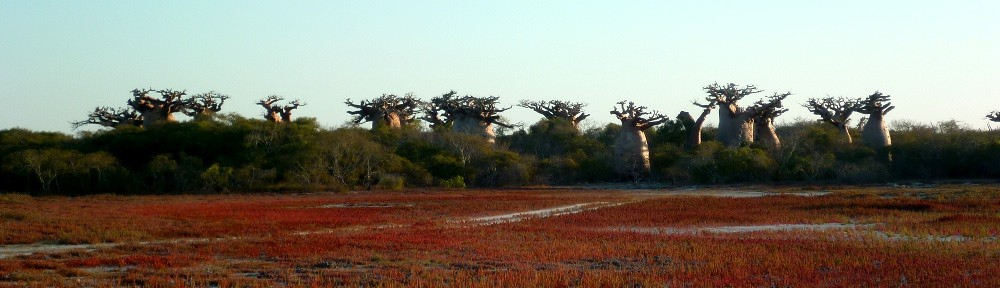
\includegraphics[width=\textwidth]{header.jpg}\\
  \textit{Adansonia grandidieri} Baill. next to Andavadoaka village (southwest Madagascar).
\end{center}

\vspace{0.5cm}

\begin{center}
  \large{
    Ghislain Vieilledent$^{\star,1}$ \hspace{0.75cm} Cory Merow$^{2}$ \hspace{0.75cm} Jérôme
    Guélat$^{3}$ \\
    \vspace{0.25cm}
    Andrew M. Latimer$^{4}$ \hspace{0.75cm} Marc Kéry$^{3}$ \\ 
    \vspace{0.25cm}
    Alan E. Gelfand$^{5}$ \hspace{0.75cm} Adam M. Wilson$^{6}$ \hspace{0.75cm}
    Frédéric Mortier$^{1}$ \\
    \vspace{0.25cm} and \hspace{0.75cm} John A. Silander Jr.$^{2}$
  }
\end{center}

\vspace{0.5cm}

%% {\footnotesize
%% \begin{flushleft}
%%   \textbf{Type of article:} Data paper for \textit{Annals of Forest Science}\\
%%   \textbf{Thematic issue:} GlobAllomeTree web platform\\
%%   \textbf{Running title:} Cirad wood density data base\\
%%   \textbf{Number of words and objects:} whole manuscript (X words) with abstract (X words),
%%   main text (X words), references (X, X words), table and figure legends (X, X words)\\
%% \end{flushleft}}

%\vspace{0.2cm}

{\footnotesize
  \begin{flushleft}
    $[\star]$ \textbf{Corresponding author:}
    \textbackslash{E-mail}:~ghislain.vieilledent@cirad.fr
    \textbackslash{Phone}:~+33.(0)4.67.59.37.51
    \textbackslash{Fax}:~+33.(0)4.67.59.39.09\\
    $[1]$ \textbf{Cirad} -- UPR BSEF, F–34398 Montpellier, France\\
    $[2]$ \textbf{University of Connecticut} -- Department of Ecology and Evolutionary
    Biology, Storrs, CT 06269, USA\\
    $[3]$ \textbf{Swiss Ornithological Institute} -- 6204 Sempach, Switzerland\\
    $[4]$ \textbf{University of California} -- Department of Plant Sciences, Davis,
    CA 95616, USA\\
    $[5]$ \textbf{Duke University} -- Department of Statistical Science, Durham, NC 27708, USA\\
    $[6]$ \textbf{Yale University} -- Department of Ecology and Evolutionary Biology, New Haven, CT 06520, USA\\
\end{flushleft}}

\newpage
%\doublespacing
%\linenumbers

\renewcommand{\abstractname}{Abstract}
\newcommand{\keywords}[1]{\par\noindent
{\small{\em Keywords\/}: #1}}

\begin{abstract}

  Species distribution models (SDM) are useful tools to explain or predict species range
  from various environmental factors. SDM are thus widely used in conservation
  biology. Based on the observations of the species in the field (occurence or
  abundance data), SDM face two major problems which lead to bias in models' results:
  imperfect detection and spatial correlation of the observations. 
  
  At the present time, there is a lack of statistical tools to analyse large occurence or
  abundance data-sets (typically with tens of hundreds observation points) taking into
  account both imperfect detection and spatial correlation.
  
  Here, we present the \textbf{hSDM} R package wich aims at providing user-friendly
  statistical functions to fill this gap. Functions were developped through a hierarchical
  Bayesian approach. They call a Metropolis-within-Gibbs algorithm coded in C to estimate
  model's parameters. Using compiled C code for the Gibbs sampler reduce drastically the
  computation time.

  By making these new statistical tools available to the scientific community, we hope to
  democratize the use of more complex, but more realistic, statistical models for
  increasing knowledge in ecology and conserving biodiversity.
  
  \vspace{0.5cm}

  \keywords{R, C code, site-occupancy models, CAR process, spatial autocorrelation,
    biodiversity, SDM, niche modelling, detection probability, counts data,
    presence-absence, false absence, uncertainty, hierachical Bayesian models, Metropolis,
    MCMC, Gibbs sampler}

\end{abstract}

\newpage

%%=============================
%% Change default shunk options



\section{Introduction}

\subsection{Species distribution models}

Biogeography is the study of the distribution of species over space and time and
biogeographers try to understand the factors determining a species distribution
\citep{Smith1868,Wallace1876}. A species distribution is often represented with a map
\citep{Wallace1876}. This knowledge on the ecology of the species can be used for several
applications such as conservation biology \citep{Thuiller2014}.

Species distribution modelling (alternatively known as ``environmental niche modelling'',
``ecological niche modelling'', ``predictive habitat distribution modelling'', and
``climate envelope modelling'') refers to the process of using computer algorithms to
predict the distribution of species in geographic space on the basis of a mathematical
representation of their known distribution in environmental space (i.e. the realized
ecological niche). The environment is in most cases represented by climate data (such as
temperature, and precipitation), but other variables such as soil type and land cover can
also be used. Species distribution models (SDM) allow estimating the probability of
presence or abundance of a species on a large geographical range using a limited number of
species observations \citep{Guisan2000, Elith2009}. Species observations can be occurence
data (presence-absence data or presence only data) or abundance data (also known as count
data).

\subsection{Imperfect detection and spatial correlation of the observations}

When considering presence-absence or abundance data for species distribution modelling,
strong assumptions are usually made \citep{Guisan2005,Sinclair2010,Araujo2006}. Among
these assumptions, two can lead to biased estimates of species distribution. The first one
deals with imperfect detection and the second one with spatial correlation of the
observations.

Regarding imperfect detection, occurrence of a species is typically not observed
perfectly. Species traits, survey-specific conditions and site-specific characteristics
may influence species detection probability which is often $<1$ \citep{Chen2013}. Thus,
observations might include false absences. For example, the habitat can be suitable and
the species is present but individuals have not been seen during the census. Or the
habitat can be suitable but the species has not dispersed yet to the site (typical example
for plant species, see \citet{Latimer2006}) or was not present on the site at the moment
of the observation (typical example for animal species such as birds, see
\citet{Kery2005}). Treating observed occurrence and species distributions as the true
occurrence and distribution, failing to make amendments for imperfect detection, may lead
to problems in species distribution studies, habitat models and biodiversity management
\citep{Latimer2006,Lahoz-Monfort2014,Kery2008}.

Regarding spatial correlation, most species present geographical patchiness (positive
spatial autocorrelation). This pattern is often driven by multiple causes that may be
associated to exogenous environmental factors such as climate or soil (which might be
partly taken into account in species distribution models), but also to endogeneous biotic
processes, called contagious processes, such as dispersal, migration, conspecific
attraction or mortality which are rarely considered
\citep{Sokal1978b,Legendre1993b,Lichstein2002,Dormann2007}. Due to the contagious biotic
processes, the presence or abundance of a species at one site is influenced by the
presence or abundance of the species at surrounding sites. A species might be present at a
site where the environment is less suitable because of the presence of the species at
neighbouring sites where the environment is higly suitable. Thus, ignoring spatial
correlation may lead to biased conclusions about ecological relationships
\citep{Lichstein2002} and even invert the slope of relationships from non-spatial analysis
in some particular cases \citep{Kuhn2006}. In addition to its ecological significance,
spatial autocorrelation is problematic for classical species distribution models which
assume independently distributed errors \citep{Legendre1993b,Lichstein2002,Dormann2007}.

\subsection{Methods and software to account for imperfect detection and spatial correlation}

New classes of models, called site-occupancy models \citep{MacKenzie2002} or zero inflated
binomial (ZIB) models \citep{Latimer2006} for presence-absence data and N-mixture models
\citep{Royle2004} or zero inflated Poisson (ZIP) models for abundance data
\citep{Flores2009}, were developed to solve the problems created by imperfect
detection. These models combine two processes, an ecological process which describes
habitat suitability and an observation process which takes into account imperfect
detection. Because they mix probability distributions to represent the suitability and
observation processes, these models have also been called mixture models. Mixture models
use information from repeated observations at several sites to estimate
detectability. Detectability may vary with site characteristics (e.g., habitat variables)
or survey characteristics (e.g., weather conditions), whereas suitability relates only to
site characteristics.

One additional point regarding site-occupancy models is that they form a unifying
framework for a very large array of capture-recapture models to estimate population size
in animal ecology \citep{Nichols1992}: using parameter-expanded data augmentation
\citep{Royle2007}, most models for population size, survival, recruitment and similar
demographic quantities (presented in detail in standard references such as
\citet{Williams2002}, \citet{Royle2008} and \citet{Kery2012}) can be cast into the
framework of an occupancy model and this makes their fitting much easier.

Several studies have demonstrated the advantages of site-occupancy and N-mixture models
over classical models which do not consider imperfect detection. These studies have
focused on the distribution of various plant or animal species in marine and terrestrial
ecosystems (see \citet{Chen2013,Latimer2006} for plants,
\citet{Kery2005,Rota2011,Dorazio2006,Royle2004} for birds, \citet{Kery2010} for insects,
\citet{Bailey2004,MacKenzie2002,Chelgren2011} for amphibians, \citet{Monk2014} for fishes,
and \citet{Poley2014,Gray2012} for mammals).

Several softwares can be used to fit site-occupancy and N-mixture models
(Table~\ref{tab:softwares-mixture}). Some are based on the maximum likelihood approach (such as
the widely used free Windows programs \textbf{MARK} and \textbf{PRESENCE} and the R
package \textbf{unmarked}) while other are based on the hierarchical Bayesian approach (such as
\textbf{WinBUGS} and \textbf{OpenBUGS} programs).

\begin{landscape}
  \begin{table}
    \begin{center}
      \begin{longtable}{@{}lrrrrL{3cm}L{3cm}R{3cm}@{}}
        \toprule
        Softwares & Socc & Nmix & Sp & Approach & OS & Reference & URL \\
        \midrule
        PRESENCE & 1 & 1 & 0 & ML & MS-W & \citet{MacKenzie2006} & \href{http://www.mbr-pwrc.usgs.gov/software/presence.html}{PRESENCE} \\
        MARK & 1 & 1 & 0 & ML & MS-W & \citet{White1999} & \href{http://www.phidot.org/software/mark/}{MARK} \\
        E-SURGE & 1 & 0 & 0 & ML & MS-W & \citet{Choquet2009} & \href{http://www.cefe.cnrs.fr/biostatistiques-et-biologie-des-populations/logiciels}{E-SURGE} \\
        unmarked & 1 & 1 & 0 & ML & cross-platform & \citet{Fiske2011} & 
        \href{http://CRAN.R-project.org/package=unmarked}{unmarked} \\
        stocc & 1 & 0 & 1 & Bayesian & cross-platform & \citet{Johnson2013} & \href{http://CRAN.R-project.org/package=stocc}{stocc} \\
        JAGS & 1 & 1 & 0 & Bayesian & cross-platform & ~ & \href{http://mcmc-jags.sourceforge.net/}{JAGS} \\
        Stan & 1 & 1 & 0 & Bayesian & cross-platform & \citet{Stan2014} & \href{http://mc-stan.org}{Stan} \\
        WinBUGS & 1 & 1 & 1 & Bayesian & MS-W & \citet{Lunn2009} & \href{http://www.mrc-bsu.cam.ac.uk/software/bugs/the-bugs-project-winbugs/}{WinBUGS} \\
        OpenBUGS & 1 & 1 & 1 & Bayesian & cross-platform & \citet{Lunn2009} & \href{http://www.openbugs.net}{OpenBUGS}\\
        hSDM & 1 & 1 & 1 & Bayesian & cross-platform & ~ & \href{http://hSDM.sf.net}{hSDM}\\
        \bottomrule
      \end{longtable}
    \end{center}
    \caption{\textbf{Softwares available for modeling species distribution including
        imperfect detection.}}
    \label{tab:softwares-mixture} 
  \end{table}
\end{landscape}

A variety of methods have been developed to correct for the effects of spatial
autocorrelation in species distribution models based on occurence or abundance data
\citep{Cressie1993,Dormann2007,Keitt2002,Miller2007}. In their review article,
\citet{Dormann2007} described six different statistical approaches to account for spatial
autocorrelation: autocovariate regression; spatial eigenvector mapping; generalised least
squares; autoregressive models and generalised estimating equations. 

Several studies have demonstrated the advantages of these mehods focusing on a variety of
plant or animal species (see \citet{Latimer2006,Gelfand2005,Kuhn2006} for plants,
\citet{Lichstein2002} for birds, and \citet{Poley2014,Johnson2013} for mammals).

Among the methods available to account for spatial autocorrelation, conditional
autoregressive (CAR) models, which incorporate spatial autocorrelation through a
neighbourhood structure, are commonly implemented in statistical softwares
\citep{Dormann2007}. The most commonly used softwares to implement CAR models are
\textbf{OpenBUGS} and \textbf{WinBUGS} softwares \citep{Lunn2009} which have in-built
functions (\texttt{car.normal} and \texttt{car.proper}) to describe the CAR process. CAR
models can also be implemented in \textbf{BayesX} \citep{Brezger2005} and in the following
R packages: \textbf{R-INLA} \citep{Rue2009}, \textbf{CARBayes} \citep{Lee2013},
\textbf{stocc} (for binary data only), \textbf{spatcounts} (for count data only),
\textbf{CARramps} (for Gaussian data only), and \textbf{spdep} (for Gaussian data only)
(Table~\ref{tab:softwares-spatial}).

\begin{landscape}
  \begin{table}
    \begin{center}
      \begin{longtable}{@{}lrrL{3cm}L{3cm}R{3cm}@{}}
        \toprule
        Softwares & Type of data & Approach & OS & Reference & URL \\
        \midrule
        OpenBUGS & all & Bayesian & cross-platform & \citet{Lunn2009} &
        \href{http://www.openbugs.net}{OpenBUGS}\\
        WinBUGS & all & Bayesian & MS-W & \citet{Lunn2009} & 
        \href{http://www.mrc-bsu.cam.ac.uk/software/bugs/the-bugs-project-winbugs/}{WinBUGS} \\
        BayesX & all & Bayesian & cross-platform & \citet{Brezger2005} &
        \href{http://www.stat.uni-muenchen.de/~bayesx/bayesx.html}{BayesX} \\ 
        R-INLA & all & Bayesian & cross-platform & \citet{Rue2009} & \href{http://www.r-inla.org/}{R-INLA} \\
        CARBayes & all & Bayesian & cross-platform & \citet{Lee2013} &
        \href{http://CRAN.R-project.org/package=CARBayes}{CARBayes} \\
        stocc & all & Bayesian & cross-platform & \citet{Johnson2013} & 
        \href{http://CRAN.R-project.org/package=stocc}{stocc} \\ 
        spatcounts & count & Bayesian & cross-platform & ~ &
        \href{http://CRAN.R-project.org/package=spatcounts}{spatcounts} \\
        CARramps & Gaussian & Bayesian & cross-platform & ~ & 
        \href{http://CRAN.R-project.org/package=CARramps}{CARramps}\\
        spdep & Gaussian & ML & cross-platform & ~ &
        \href{http://CRAN.R-project.org/package=spdep}{spdep} \\
        hSDM & binomial and count & Bayesian & cross-platform & ~ & \href{http://hSDM.sf.net}{hSDM}\\
        \bottomrule
      \end{longtable}
    \end{center}
    \caption{\textbf{Softwares available for modeling species distribution including
        spatial autocorrelation.}}
    \label{tab:softwares-spatial} 
  \end{table}
\end{landscape}

\subsection{Objectives of the hSDM R package}

Among the available statistical programs, only \textbf{OpenBUGS} can be used on any
operating system to fit both site-occupancy or N-mixture models including also a spatial
autocorrelation process (Table~\ref{tab:softwares-mixture} and
Table~\ref{tab:softwares-spatial}). One problem is that \textbf{OpenBUGS}, for such
models, cannot handle large data-sets (typically, data-sets with tens of thousands
sites). Moreover, for smaller data-sets, models can be fitted but computation time can be
long due to the fact that the \textbf{OpenBUGS} code is interpreted and not compiled. For
this reason, we decided to develop the \textbf{hSDM} (for hierarchical Bayesian species
distribution models) R package. The \textbf{stocc} R package
\citep{Johnson2013,Poley2014}, which can handle binary data only, has been developed for
the same reasons. The \textbf{hSDM} package allows the user to fit mixture models which
take into account imperfect detection (site-occupancy, N-mixture, ZIB and ZIP models) and
account for spatial autocorrelation. Spatial autocorrelation is represented through an
intrinsic CAR process \citep{Besag1991}. Functions in the \textbf{hSDM} R package use a
Metropolis algorithm \citep{Robert2004} in a Gibbs sampler \citep{Casella1992,
  Gelfand1990} to obtain the posterior distribution of model's parameters. The Gibbs
sampler is written in C code and compiled to optimize computation efficiency. Thus, the
\textbf{hSDM} package can be used for very large data-sets while reducing drastically the
computation time.

In this vignette, we present examples to illustrate the use of the \textbf{hSDM} package
in the R statistical environment \citep{R2014}. Examples use virtual or real
data-sets. Results obtained with functions in the \textbf{hSDM} package are compared with
the results obtained with other softwares and models.

\newpage

\section{Species distribution models}

\subsection{Binomial model}
\label{sec:binomial}

\subsubsection{Mathematical formulation}

Let's consider a random variable $y_i$ representing the total number of presences of a
species after several visits $v_i$ at a particular site $i$. Random variable $y_i$ can
take values from 0 to $v_i$ and can be assumed to follow a Binomial distribution having
parameters $v_i$ and $\theta_i$ (Eq.~\ref{eq:binomial}). Parameter $\theta_i$ can be
interpreted as the probability of presence of the species at site $i$ . Using a logit link
function, $\theta_i$ can be expressed as a linear model combining explicative variables
$X_i$ and parameters $\beta$ (Eq.~\ref{eq:binomial}).

\begin{equation}
  \begin{tabular}{c}
    $y_i \sim \mathcal{B}inomial(v_i,\theta_i)$ \\
    ~ \\
    $\logit(\theta_i) = X_i \beta$ \\
  \end{tabular}
  \label{eq:binomial}
\end{equation}

Using this statistical model, we aim at representing a ``suitability process''. Given
environmental variables $X_i$, how much is habitat at site $i$ suitable for the species
under consideration? Parameters $\beta$ indicate how much each environmental variable
contributes to the suitability process. Like every other function in the \textbf{hSDM} R
package, function \texttt{hSDM.binomial()} estimates the parameters $\beta$ of such a
model in a Bayesian framework. Parameter inference is done using a Gibbs sampler including
a Metropolis algorithm. The Gibbs sampler is coded in the C language to optimize
computation efficiency.

\subsubsection{Data generation}

To explore the characteristics of the \texttt{hSDM.binomial()} function, we can generate a
virtual data-set on the basis of the Binomial model described above
(Eq.~\ref{eq:binomial}). In the most general case (presence/absence data or
presence/background data), a site $i$ is visited once and $v_i=1$. Thus, the random
variable $y_i$ follows a Bernoulli distribution having parameters $\theta_i$ and habitat
characteristics $X_i$ are fixed for site $i$. We will generate a virtual data-set in this
particular case. For data generation, we can import virtual altitudinal data in
R. Altitude will be used as an explicative variable to determine habitat suitability,
i.e. the probability of presence of a virtual species. Altitudinal data are loaded at the
same time as the \textbf{hSDM} R package (data frame \texttt{altitude} in the working
directory).

These data can be transformed into a raster object using the function
\texttt{rasterFromXYZ()} from the \textbf{raster} package. The raster has 2500 cells (50
columns and 50 rows) and the altitude ranges roughly between 100 and 600~m
(Fig.~\ref{fig:Altitude}). For linear models, explicative variables are usually centered
and scaled to facilitate inference and interpretation of model parameters.

\begin{knitrout}\small
\definecolor{shadecolor}{rgb}{0.969, 0.969, 0.969}\color{fgcolor}\begin{kframe}
\begin{alltt}
\hlcom{# Load altitudinal data and create raster}
\hlkwd{library}\hlstd{(raster)}
\hlkwd{data}\hlstd{(altitude,}\hlkwc{package}\hlstd{=}\hlstr{"hSDM"}\hlstd{)}
\hlstd{alt.orig} \hlkwb{<-} \hlkwd{rasterFromXYZ}\hlstd{(altitude)}
\hlkwd{extent}\hlstd{(alt.orig)} \hlkwb{<-} \hlkwd{c}\hlstd{(}\hlnum{0}\hlstd{,}\hlnum{50}\hlstd{,}\hlnum{0}\hlstd{,}\hlnum{50}\hlstd{)}
\hlkwd{plot}\hlstd{(alt.orig)}
\hlcom{# Center and scale altitudinal data}
\hlstd{alt} \hlkwb{<-} \hlkwd{scale}\hlstd{(alt.orig,}\hlkwc{center}\hlstd{=}\hlnum{TRUE}\hlstd{,}\hlkwc{scale}\hlstd{=}\hlnum{TRUE}\hlstd{)}
\hlkwd{plot}\hlstd{(alt)}
\end{alltt}
\end{kframe}
\end{knitrout}


\begin{figure} 
  \begin{tabular}{cc}
    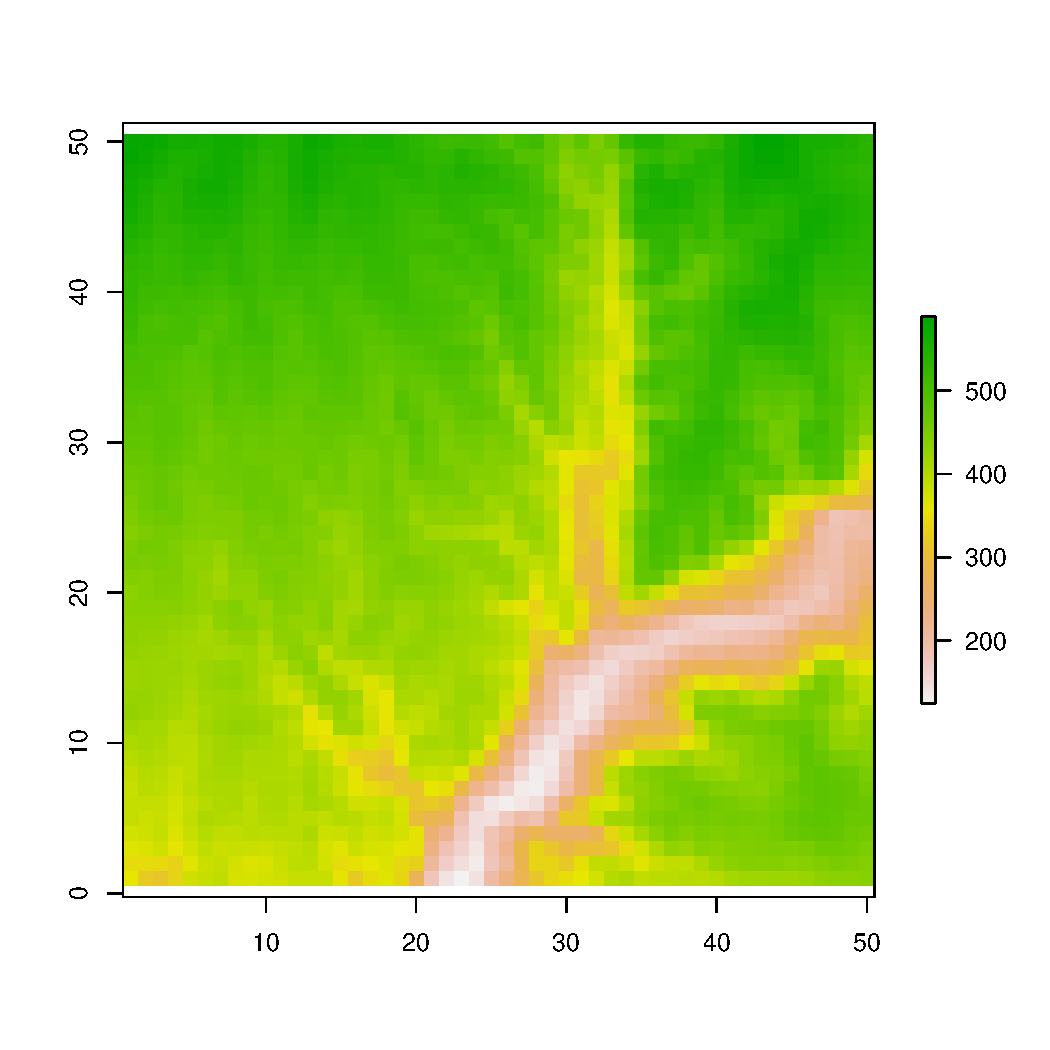
\includegraphics[width=8cm]{figures/Altitude1.pdf} &
    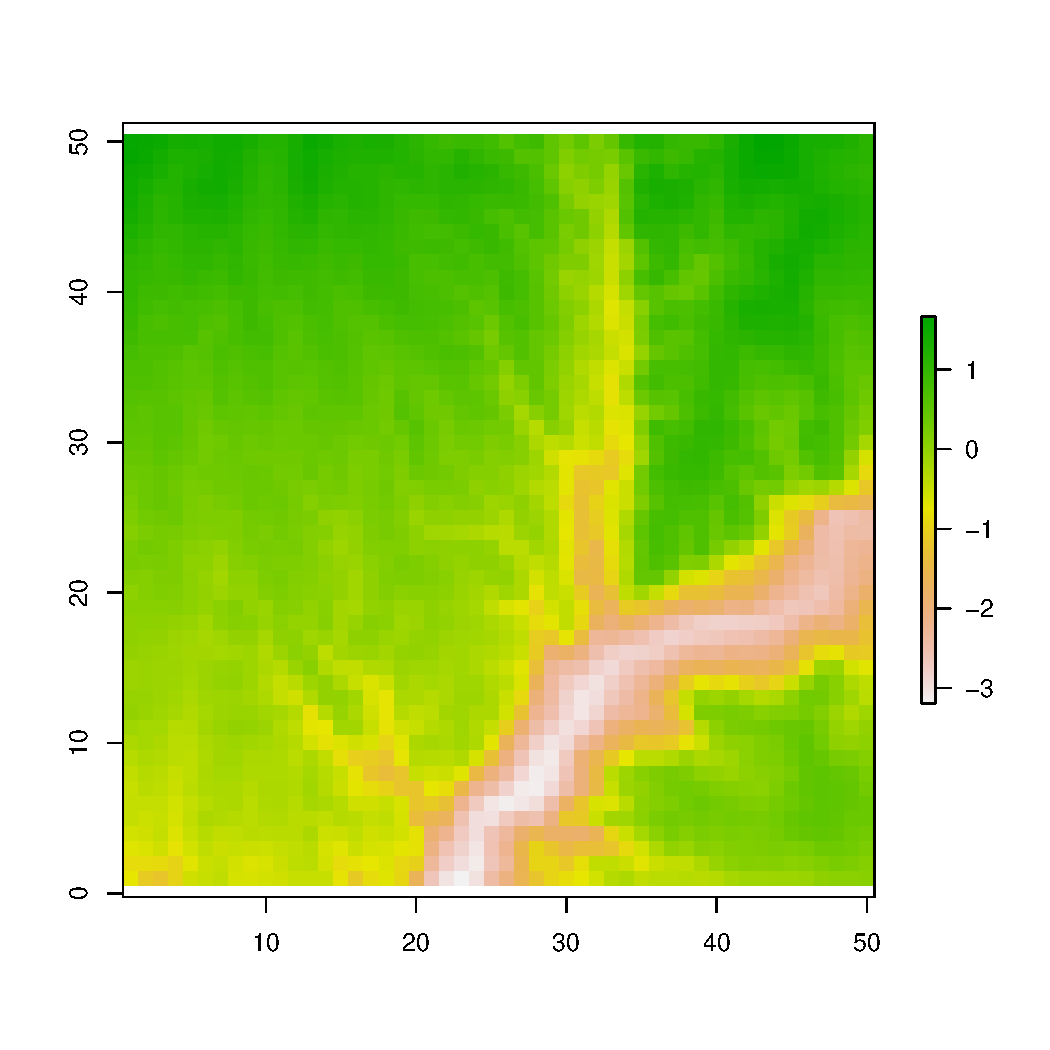
\includegraphics[width=8cm]{figures/Altitude2.pdf} \\
  \end{tabular}
  \caption{\textbf{Altitudinal data}. Original values (in m) on the left. Centered and
    scaled values on the right.}
  \label{fig:Altitude}
\end{figure}

A linear model including altitude (variable denoted $A$) is used to compute the
probability of presence of the species (Eq.~\ref{eq:bernoulli}).

\begin{equation}
  \begin{tabular}{c}
    $y_i \sim \mathcal{B}ernoulli(\theta_i)$ \\
    ~ \\
    $\logit(\theta_i) = \beta_0 + \beta_1 A_i$ \\
  \end{tabular}
  \label{eq:bernoulli}
\end{equation}

We fix the parameters to $\beta_0=-1$ and $\beta_1=1$. The species has a higher
probability of presence at higher altitudes (Fig.~\ref{fig:theta-binomial}).

\begin{knitrout}\small
\definecolor{shadecolor}{rgb}{0.969, 0.969, 0.969}\color{fgcolor}\begin{kframe}
\begin{alltt}
\hlcom{# Load hSDM library}
\hlkwd{library}\hlstd{(hSDM)}
\hlcom{# Target parameters}
\hlstd{beta.target} \hlkwb{<-} \hlkwd{matrix}\hlstd{(}\hlkwd{c}\hlstd{(}\hlopt{-}\hlnum{1}\hlstd{,}\hlnum{1}\hlstd{),}\hlkwc{ncol}\hlstd{=}\hlnum{1}\hlstd{)}
\hlcom{# Matrix of covariates (including the intercept)}
\hlstd{ncells} \hlkwb{<-} \hlkwd{ncell}\hlstd{(alt)}
\hlstd{X} \hlkwb{<-} \hlkwd{cbind}\hlstd{(}\hlkwd{rep}\hlstd{(}\hlnum{1}\hlstd{,ncells),}\hlkwd{values}\hlstd{(alt))}
\hlcom{# Probability of presence as a quadratic function of altitude}
\hlstd{logit.theta} \hlkwb{<-} \hlstd{X} \hlopt \hlstd{beta.target}
\hlstd{theta} \hlkwb{<-} \hlkwd{inv.logit}\hlstd{(logit.theta)}
\hlcom{# Coordinates of raster cells}
\hlstd{coords} \hlkwb{<-} \hlkwd{coordinates}\hlstd{(alt)}
\hlcom{# Transform the probability of presence into a raster}
\hlstd{theta} \hlkwb{<-} \hlkwd{rasterFromXYZ}\hlstd{(}\hlkwd{cbind}\hlstd{(coords,theta))}
\hlcom{# Color palette for probability plots}
\hlstd{colRP} \hlkwb{<-} \hlkwd{colorRampPalette}\hlstd{(}\hlkwd{c}\hlstd{(}\hlstr{"white"}\hlstd{,}\hlstr{"yellow"}\hlstd{,}\hlstr{"orange"}\hlstd{,}
                            \hlstr{"red"}\hlstd{,}\hlstr{"brown"}\hlstd{,}\hlstr{"black"}\hlstd{))}
\hlcom{# Plot the probability of presence}
\hlstd{brks} \hlkwb{<-} \hlkwd{seq}\hlstd{(}\hlnum{0}\hlstd{,}\hlnum{1}\hlstd{,}\hlkwc{length.out}\hlstd{=}\hlnum{100}\hlstd{)}
\hlstd{arg} \hlkwb{<-} \hlkwd{list}\hlstd{(}\hlkwc{at}\hlstd{=}\hlkwd{seq}\hlstd{(}\hlnum{0}\hlstd{,}\hlnum{1}\hlstd{,}\hlkwc{length.out}\hlstd{=}\hlnum{5}\hlstd{),} \hlkwc{labels}\hlstd{=}\hlkwd{c}\hlstd{(}\hlstr{"0"}\hlstd{,}\hlstr{"0.25"}\hlstd{,}\hlstr{"0.5"}\hlstd{,}\hlstr{"0.75"}\hlstd{,}\hlstr{"1"}\hlstd{))}
\hlstd{nb} \hlkwb{<-} \hlkwd{length}\hlstd{(brks)}\hlopt{-}\hlnum{1}
\hlkwd{plot}\hlstd{(theta,}\hlkwc{main}\hlstd{=}\hlstr{"Initial probabilities"}\hlstd{,}\hlkwc{col}\hlstd{=}\hlkwd{colRP}\hlstd{(nb),}
     \hlkwc{breaks}\hlstd{=brks,}\hlkwc{axis.args}\hlstd{=arg,}\hlkwc{zlim}\hlstd{=}\hlkwd{c}\hlstd{(}\hlnum{0}\hlstd{,}\hlnum{1}\hlstd{))}
\end{alltt}
\end{kframe}
\end{knitrout}


\begin{figure} 
  \centering 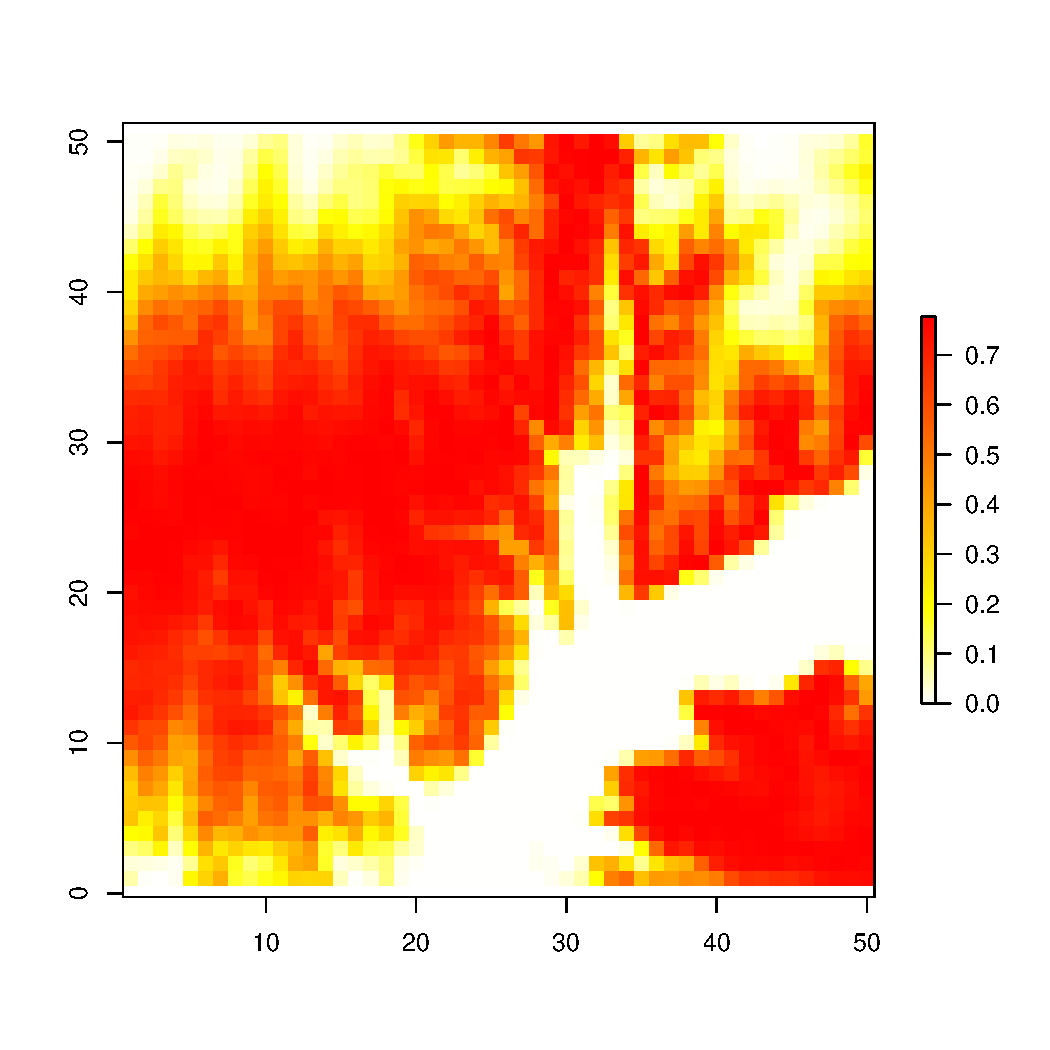
\includegraphics[width=8cm]{figures/theta-binomial.pdf}
  \caption{\textbf{Probability of presence}.}
  \label{fig:theta-binomial}
\end{figure}

We can assume a number $n$ of sites in the landscape where we have been able to observe
or not the presence of the species. We can simulate the presence or absence of the species
at these $n$ sites given our model (Fig.~\ref{fig:observations-binomial}).

\begin{knitrout}\small
\definecolor{shadecolor}{rgb}{0.969, 0.969, 0.969}\color{fgcolor}\begin{kframe}
\begin{alltt}
\hlcom{# Number of observation sites}
\hlstd{nsite} \hlkwb{<-} \hlnum{200}
\hlcom{# Set seed for repeatability}
\hlstd{seed} \hlkwb{<-} \hlnum{1234}
\hlcom{# Sample the observations in the landscape}
\hlkwd{set.seed}\hlstd{(seed)}
\hlstd{x.coord} \hlkwb{<-} \hlkwd{runif}\hlstd{(nsite,}\hlnum{0}\hlstd{,}\hlnum{50}\hlstd{)}
\hlkwd{set.seed}\hlstd{(}\hlnum{2}\hlopt{*}\hlstd{seed)}
\hlstd{y.coord} \hlkwb{<-} \hlkwd{runif}\hlstd{(nsite,}\hlnum{0}\hlstd{,}\hlnum{50}\hlstd{)}
\hlkwd{library}\hlstd{(sp)}
\hlstd{sites.sp} \hlkwb{<-} \hlkwd{SpatialPoints}\hlstd{(}\hlkwc{coords}\hlstd{=}\hlkwd{cbind}\hlstd{(x.coord,y.coord))}
\hlcom{# Extract altitude data for sites}
\hlstd{alt.sites} \hlkwb{<-} \hlkwd{extract}\hlstd{(alt,sites.sp)}
\hlcom{# Compute theta for these observations}
\hlstd{X.sites} \hlkwb{<-} \hlkwd{cbind}\hlstd{(}\hlkwd{rep}\hlstd{(}\hlnum{1}\hlstd{,nsite),alt.sites)}
\hlstd{logit.theta.site} \hlkwb{<-} \hlstd{X.sites} \hlopt \hlstd{beta.target}
\hlstd{theta.site} \hlkwb{<-} \hlkwd{inv.logit}\hlstd{(logit.theta.site)}
\hlcom{# Simulate observations}
\hlstd{visits} \hlkwb{<-} \hlkwd{rep}\hlstd{(}\hlnum{1}\hlstd{,nsite)} \hlcom{# One visit per site for the moment}
\hlkwd{set.seed}\hlstd{(seed)}
\hlstd{Y} \hlkwb{<-} \hlkwd{rbinom}\hlstd{(nsite,visits,theta.site)}
\hlcom{# Group explicative and response variables in a data-frame}
\hlstd{data.obs.df} \hlkwb{<-} \hlkwd{data.frame}\hlstd{(Y,visits,}\hlkwc{alt}\hlstd{=X.sites[,}\hlnum{2}\hlstd{])}
\hlcom{# Transform observations in a spatial object}
\hlstd{data.obs} \hlkwb{<-} \hlkwd{SpatialPointsDataFrame}\hlstd{(}\hlkwc{coords}\hlstd{=}\hlkwd{coordinates}\hlstd{(sites.sp),}
                                   \hlkwc{data}\hlstd{=data.obs.df)}
\hlcom{# Plot observations}
\hlkwd{plot}\hlstd{(alt.orig)}
\hlkwd{points}\hlstd{(data.obs[data.obs}\hlopt{$}\hlstd{Y}\hlopt{==}\hlnum{1}\hlstd{,],}\hlkwc{pch}\hlstd{=}\hlnum{16}\hlstd{)}
\hlkwd{points}\hlstd{(data.obs[data.obs}\hlopt{$}\hlstd{Y}\hlopt{==}\hlnum{0}\hlstd{,],}\hlkwc{pch}\hlstd{=}\hlnum{1}\hlstd{)}
\end{alltt}
\end{kframe}
\end{knitrout}


\begin{figure} 
  \centering 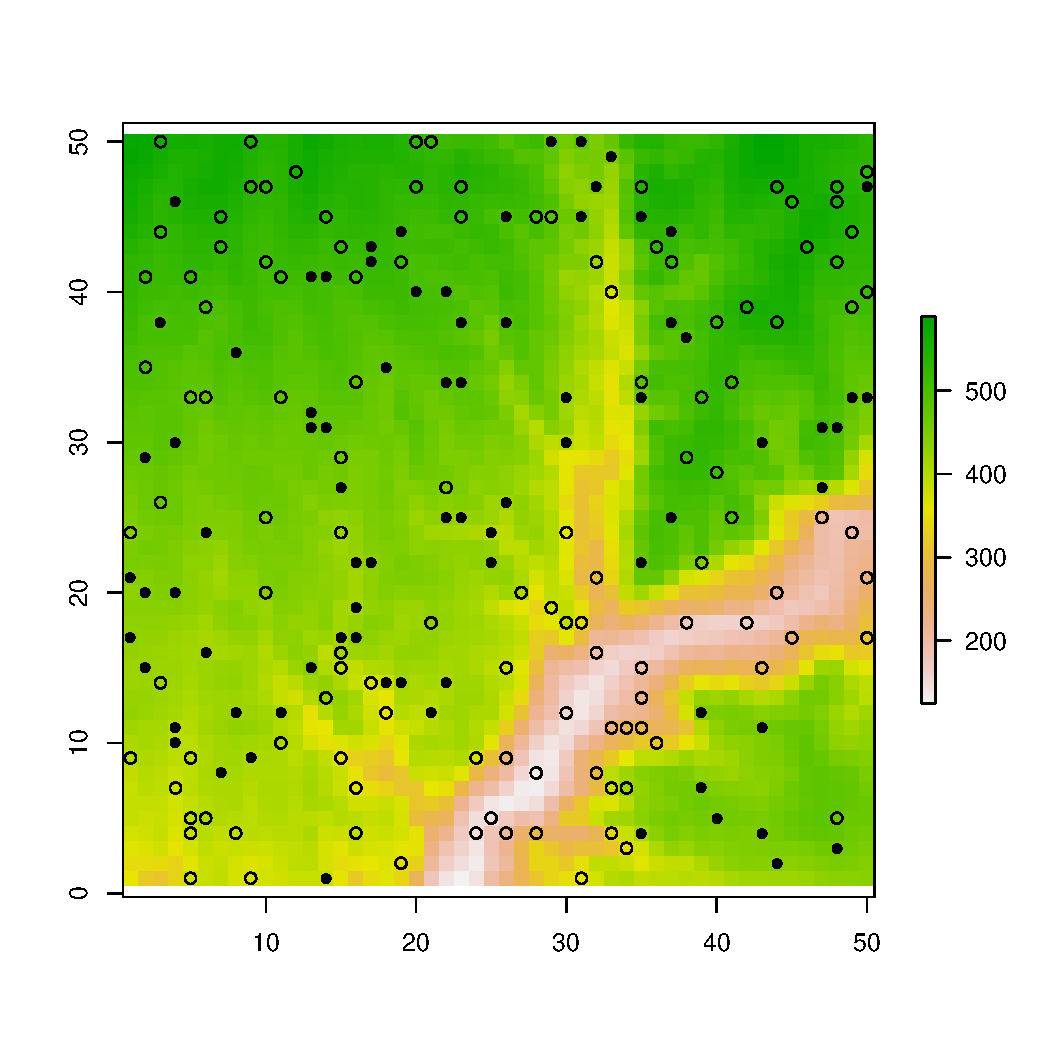
\includegraphics[width=8cm]{figures/observations-binomial.pdf}
  \caption{\textbf{Observation points}. Presences (full circles) and absences (empty
    circles) are localized on the altitude map (in m).}
  \label{fig:observations-binomial}
\end{figure}

\subsubsection{Parameter inference using the \texttt{hSDM.binomial()} function}

The \texttt{hSDM.binomial()} function performs a Binomial logistic regression in a
Bayesian framework. Before using this function we need to prepare a bit the data for
predictions. We want to have predictions on the whole landscape, not only at observation
points. To directly obtain these predictions, we can create a data frame including
altitudinal data on the whole landscape. This data frame will be used for the
\texttt{suitability.pred} argument. The data frame for predictions must include the same
column names as those used in the formula for the \texttt{suitability} argument
(i.e. ``alt'' our example).

\begin{knitrout}\small
\definecolor{shadecolor}{rgb}{0.969, 0.969, 0.969}\color{fgcolor}\begin{kframe}
\begin{alltt}
\hlstd{data.pred} \hlkwb{<-} \hlkwd{data.frame}\hlstd{(}\hlkwc{alt}\hlstd{=}\hlkwd{values}\hlstd{(alt))}
\end{alltt}
\end{kframe}
\end{knitrout}


We can now call the \texttt{hSDM.binomial()} function. Setting parameter \texttt{save.p}
to 1, we can save in memory the MCMC values for predictions. These values can be used to compute
several statistics for each predictions (mean, median, 95\% quantiles). For example, mean
and 95\% quantiles are useful to estimate the uncertainty around the mean predictions.     

\begin{knitrout}\small
\definecolor{shadecolor}{rgb}{0.969, 0.969, 0.969}\color{fgcolor}\begin{kframe}
\begin{alltt}
\hlstd{mod.hSDM.binomial} \hlkwb{<-} \hlkwd{hSDM.binomial}\hlstd{(}\hlkwc{presences}\hlstd{=data.obs}\hlopt{$}\hlstd{Y,}
                                   \hlkwc{trials}\hlstd{=data.obs}\hlopt{$}\hlstd{visits,}
                                   \hlkwc{suitability}\hlstd{=}\hlopt{~}\hlstd{alt,}
                                   \hlkwc{data}\hlstd{=data.obs,}
                                   \hlkwc{suitability.pred}\hlstd{=data.pred,}
                                   \hlkwc{burnin}\hlstd{=}\hlnum{1000}\hlstd{,} \hlkwc{mcmc}\hlstd{=}\hlnum{1000}\hlstd{,} \hlkwc{thin}\hlstd{=}\hlnum{1}\hlstd{,}
                                   \hlkwc{beta.start}\hlstd{=}\hlnum{0}\hlstd{,}
                                   \hlkwc{mubeta}\hlstd{=}\hlnum{0}\hlstd{,} \hlkwc{Vbeta}\hlstd{=}\hlnum{1.0E6}\hlstd{,}
                                   \hlkwc{seed}\hlstd{=}\hlnum{1234}\hlstd{,} \hlkwc{verbose}\hlstd{=}\hlnum{1}\hlstd{,} \hlkwc{save.p}\hlstd{=}\hlnum{1}\hlstd{)}
\end{alltt}
\end{kframe}
\end{knitrout}


\subsubsection{Analysis of the results}

The \texttt{hSDM.binomial()} function returns an MCMC (Markov chain Monte Carlo) for each
parameter of the model and also for the model deviance. To obtain parameter estimates,
MCMC values can be summarized through a call to the \texttt{summary()} function from the
\textbf{coda} package. We can check that the values of the target parameters, $\beta_0=-1$
and $\beta_1=1$, are within the 95\% confidence interval of the parameter estimates.

\begin{knitrout}\small
\definecolor{shadecolor}{rgb}{0.969, 0.969, 0.969}\color{fgcolor}\begin{kframe}
\begin{alltt}
\hlkwd{summary}\hlstd{(mod.hSDM.binomial}\hlopt{$}\hlstd{mcmc)}
\end{alltt}
\begin{verbatim}
## 
## Iterations = 1001:2000
## Thinning interval = 1 
## Number of chains = 1 
## Sample size per chain = 1000 
## 
## 1. Empirical mean and standard deviation for each variable,
##    plus standard error of the mean:
## 
##                     Mean    SD Naive SE Time-series SE
## beta.(Intercept)  -1.413 0.226  0.00713         0.0223
## beta.alt           0.984 0.296  0.00936         0.0328
## Deviance         202.166 2.285  0.07225         0.1661
## 
## 2. Quantiles for each variable:
## 
##                     2.5%     25%     50%    75%   97.5%
## beta.(Intercept)  -1.843  -1.557  -1.413  -1.27  -0.958
## beta.alt           0.451   0.783   0.969   1.18   1.681
## Deviance         199.895 200.490 201.328 203.19 207.664
\end{verbatim}
\end{kframe}
\end{knitrout}


Parameters estimates can be compared to results obtained with the \texttt{glm()} function.

\begin{knitrout}\small
\definecolor{shadecolor}{rgb}{0.969, 0.969, 0.969}\color{fgcolor}\begin{kframe}
\begin{alltt}
\hlcom{#== glm results for comparison}
\hlstd{mod.glm} \hlkwb{<-} \hlkwd{glm}\hlstd{(}\hlkwd{cbind}\hlstd{(Y,visits}\hlopt{-}\hlstd{Y)}\hlopt{~}\hlstd{alt,}\hlkwc{family}\hlstd{=}\hlstr{"binomial"}\hlstd{,}\hlkwc{data}\hlstd{=data.obs)}
\hlkwd{summary}\hlstd{(mod.glm)}
\end{alltt}
\begin{verbatim}
## 
## Call:
## glm(formula = cbind(Y, visits - Y) ~ alt, family = "binomial", 
##     data = data.obs)
## 
## Deviance Residuals: 
##    Min      1Q  Median      3Q     Max  
## -1.129  -0.751  -0.604  -0.175   2.728  
## 
## Coefficients:
##             Estimate Std. Error z value Pr(>|z|)    
## (Intercept)   -1.382      0.197   -7.03    2e-12 ***
## alt            0.952      0.276    3.44  0.00057 ***
## ---
## Signif. codes:  0 '***' 0.001 '**' 0.01 '*' 0.05 '.' 0.1 ' ' 1
## 
## (Dispersion parameter for binomial family taken to be 1)
## 
##     Null deviance: 215.71  on 199  degrees of freedom
## Residual deviance: 199.79  on 198  degrees of freedom
## AIC: 203.8
## 
## Number of Fisher Scoring iterations: 5
\end{verbatim}
\end{kframe}
\end{knitrout}


MCMC can also be graphically summarized with a call to the \texttt{plot.mcmc()} function,
also in the \textbf{coda} package. MCMC are plotted with a trace of the sampled output and
a density estimate for each variable in the chain (Fig.~\ref{fig:mcmc-binomial}). This
plot can be used to visually check that the chains have converged.

\begin{knitrout}\small
\definecolor{shadecolor}{rgb}{0.969, 0.969, 0.969}\color{fgcolor}\begin{kframe}
\begin{alltt}
\hlkwd{plot}\hlstd{(mod.hSDM.binomial}\hlopt{$}\hlstd{mcmc)}
\end{alltt}
\end{kframe}
\end{knitrout}


\begin{figure} 
  \centering 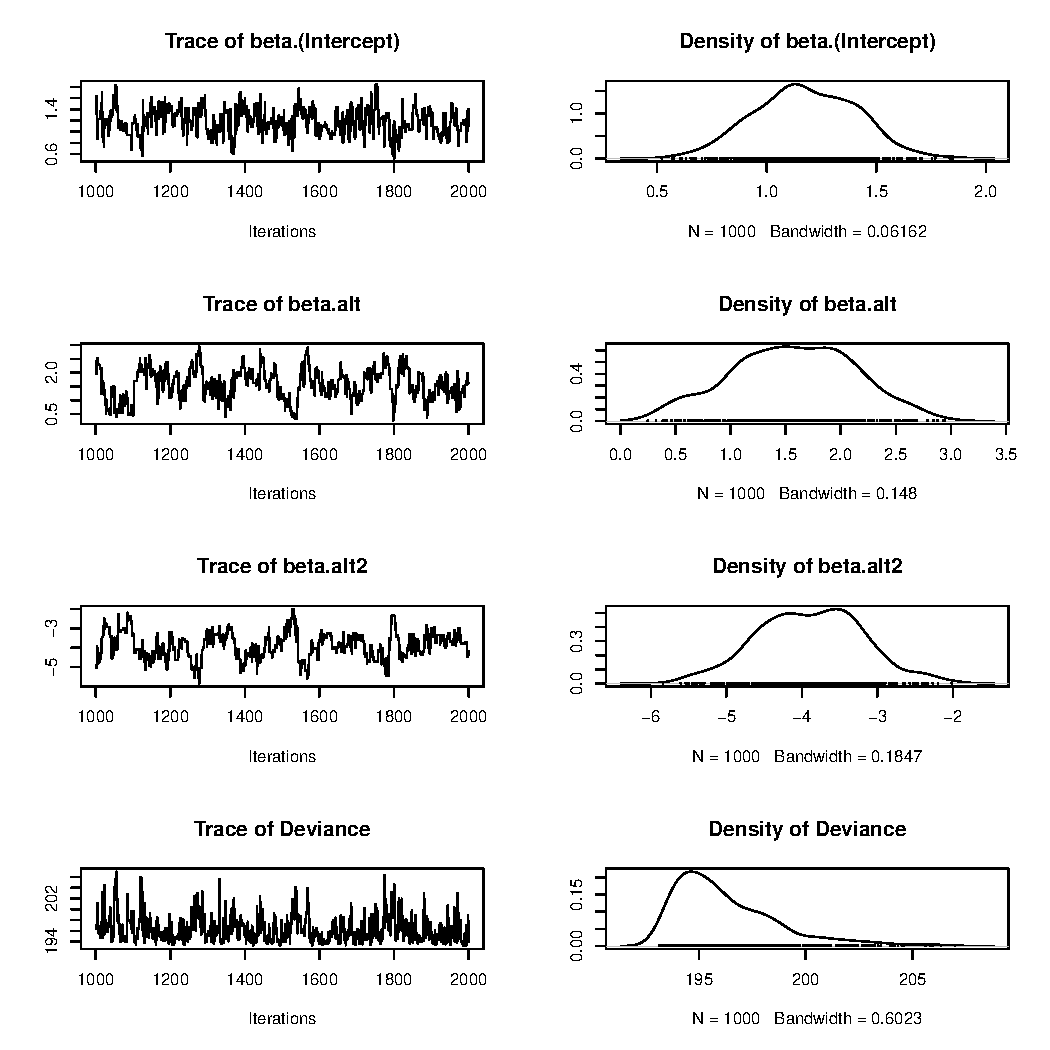
\includegraphics[width=\textwidth]{figures/mcmc-binomial.pdf}
  \caption{\textbf{Trace and density estimate for each variable of the MCMC}.}
  \label{fig:mcmc-binomial}
\end{figure}

The \texttt{hSDM.binomial()} function also returns two other objects. The first one,
\texttt{theta.latent}, is the predictive posterior mean of the latent variable
$\theta$ (the probability of presence) for each observation. 

\begin{knitrout}\small
\definecolor{shadecolor}{rgb}{0.969, 0.969, 0.969}\color{fgcolor}\begin{kframe}
\begin{alltt}
\hlkwd{str}\hlstd{(mod.hSDM.binomial}\hlopt{$}\hlstd{theta.latent)}
\end{alltt}
\begin{verbatim}
##  num [1:200] 0.2191 0.0992 0.1038 0.1878 0.221 ...
\end{verbatim}
\begin{alltt}
\hlkwd{summary}\hlstd{(mod.hSDM.binomial}\hlopt{$}\hlstd{theta.latent)}
\end{alltt}
\begin{verbatim}
##    Min. 1st Qu.  Median    Mean 3rd Qu.    Max. 
##  0.0171  0.1540  0.2180  0.2300  0.2970  0.4970
\end{verbatim}
\end{kframe}
\end{knitrout}


The second one, \texttt{theta.pred} is the set of sampled values from the predictive
posterior (if parameter \texttt{save.p} is set to 1) or the predictive posterior mean (if
\texttt{save.p} is set to 0) for each prediction. In our example, \texttt{save.p} is set
to 1 and \texttt{theta.pred} is an \texttt{mcmc} object. Values in \texttt{theta.pred} can
be used to plot the predicted probability of presence on the whole landscape and the
uncertainty associated to predictions (Fig~\ref{fig:predictions-binomial}).

\begin{knitrout}\small
\definecolor{shadecolor}{rgb}{0.969, 0.969, 0.969}\color{fgcolor}\begin{kframe}
\begin{alltt}
\hlcom{# Create a raster for predictions}
\hlstd{theta.pred.mean} \hlkwb{<-} \hlkwd{raster}\hlstd{(theta)}
\hlcom{# Create rasters for uncertainty}
\hlstd{theta.pred.2.5} \hlkwb{<-} \hlstd{theta.pred.97.5} \hlkwb{<-} \hlkwd{raster}\hlstd{(theta)}
\hlcom{# Attribute predicted values to raster cells}
\hlstd{theta.pred.mean[]} \hlkwb{<-} \hlkwd{apply}\hlstd{(mod.hSDM.binomial}\hlopt{$}\hlstd{theta.pred,}\hlnum{2}\hlstd{,mean)}
\hlstd{theta.pred.2.5[]} \hlkwb{<-} \hlkwd{apply}\hlstd{(mod.hSDM.binomial}\hlopt{$}\hlstd{theta.pred,}\hlnum{2}\hlstd{,quantile,}\hlnum{0.025}\hlstd{)}
\hlstd{theta.pred.97.5[]} \hlkwb{<-} \hlkwd{apply}\hlstd{(mod.hSDM.binomial}\hlopt{$}\hlstd{theta.pred,}\hlnum{2}\hlstd{,quantile,}\hlnum{0.975}\hlstd{)}
\hlcom{# Plot the predicted probability of presence and uncertainty}
\hlkwd{plot}\hlstd{(theta.pred.mean,}\hlkwc{main}\hlstd{=}\hlstr{"Mean"}\hlstd{,}\hlkwc{col}\hlstd{=}\hlkwd{colRP}\hlstd{(nb),}\hlkwc{breaks}\hlstd{=brks,}
     \hlkwc{axis.args}\hlstd{=arg,}\hlkwc{zlim}\hlstd{=}\hlkwd{c}\hlstd{(}\hlnum{0}\hlstd{,}\hlnum{1}\hlstd{))}
\hlkwd{plot}\hlstd{(theta.pred.2.5,}\hlkwc{main}\hlstd{=}\hlstr{"Quantile 2.5 %"}\hlstd{,}\hlkwc{col}\hlstd{=}\hlkwd{colRP}\hlstd{(nb),}\hlkwc{breaks}\hlstd{=brks,}
     \hlkwc{axis.args}\hlstd{=arg,}\hlkwc{zlim}\hlstd{=}\hlkwd{c}\hlstd{(}\hlnum{0}\hlstd{,}\hlnum{1}\hlstd{))}
\hlkwd{plot}\hlstd{(theta.pred.97.5,}\hlkwc{main}\hlstd{=}\hlstr{"Quantile 97.5 %"}\hlstd{,}\hlkwc{col}\hlstd{=}\hlkwd{colRP}\hlstd{(nb),}\hlkwc{breaks}\hlstd{=brks,}
     \hlkwc{axis.args}\hlstd{=arg,}\hlkwc{zlim}\hlstd{=}\hlkwd{c}\hlstd{(}\hlnum{0}\hlstd{,}\hlnum{1}\hlstd{))}
\end{alltt}
\end{kframe}
\end{knitrout}


\begin{figure} 
  \centering 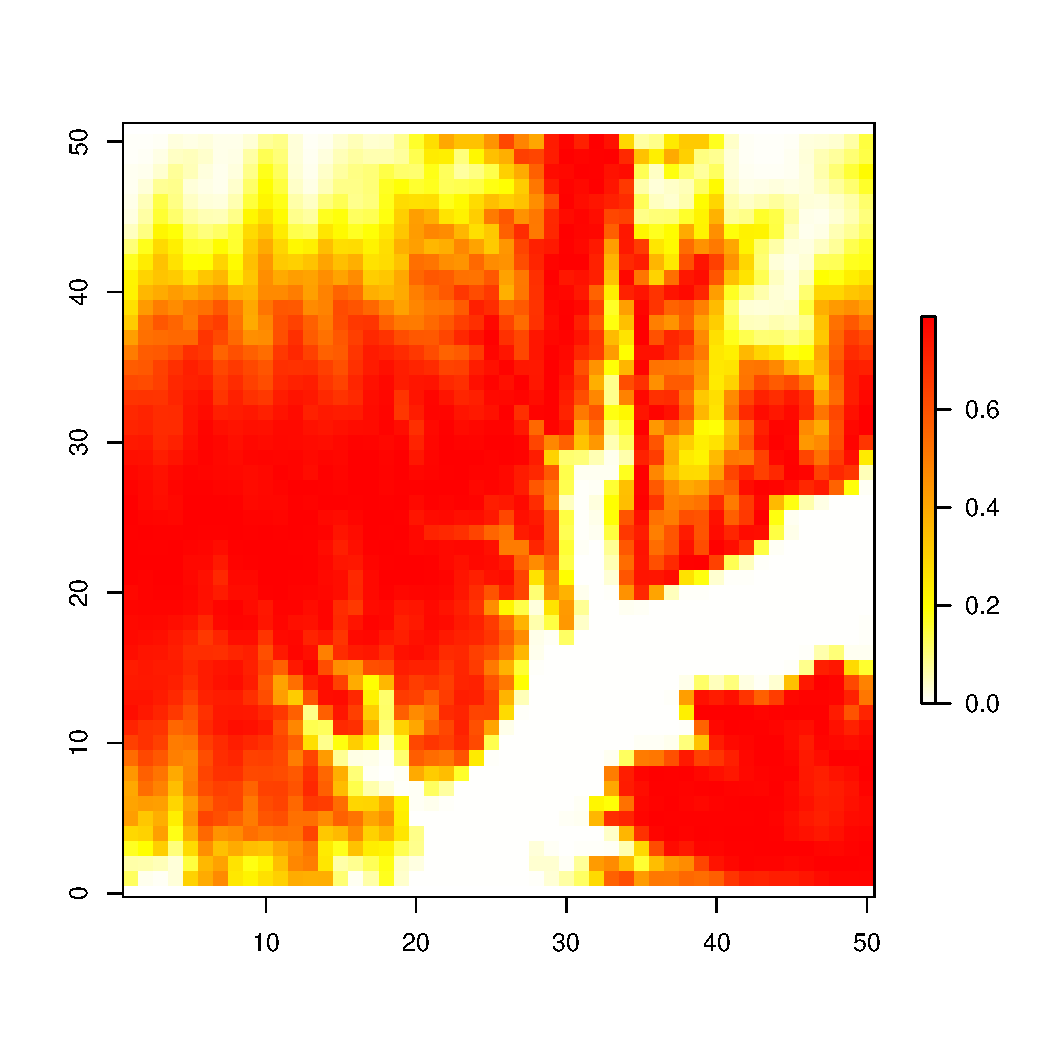
\includegraphics[width=8cm]{figures/predictions-binomial1.pdf} \\
  \begin{tabular}{cc}
    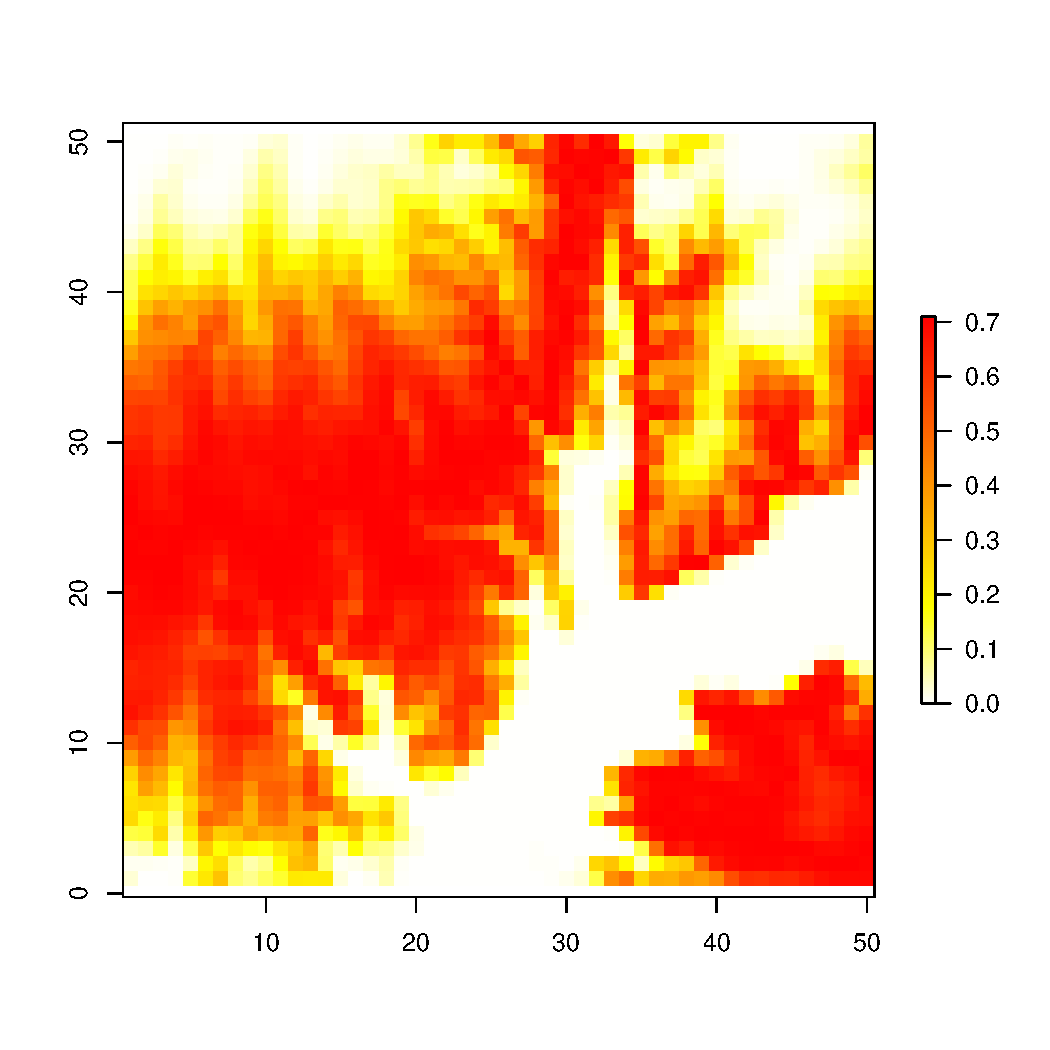
\includegraphics[width=8cm]{figures/predictions-binomial2.pdf} &
    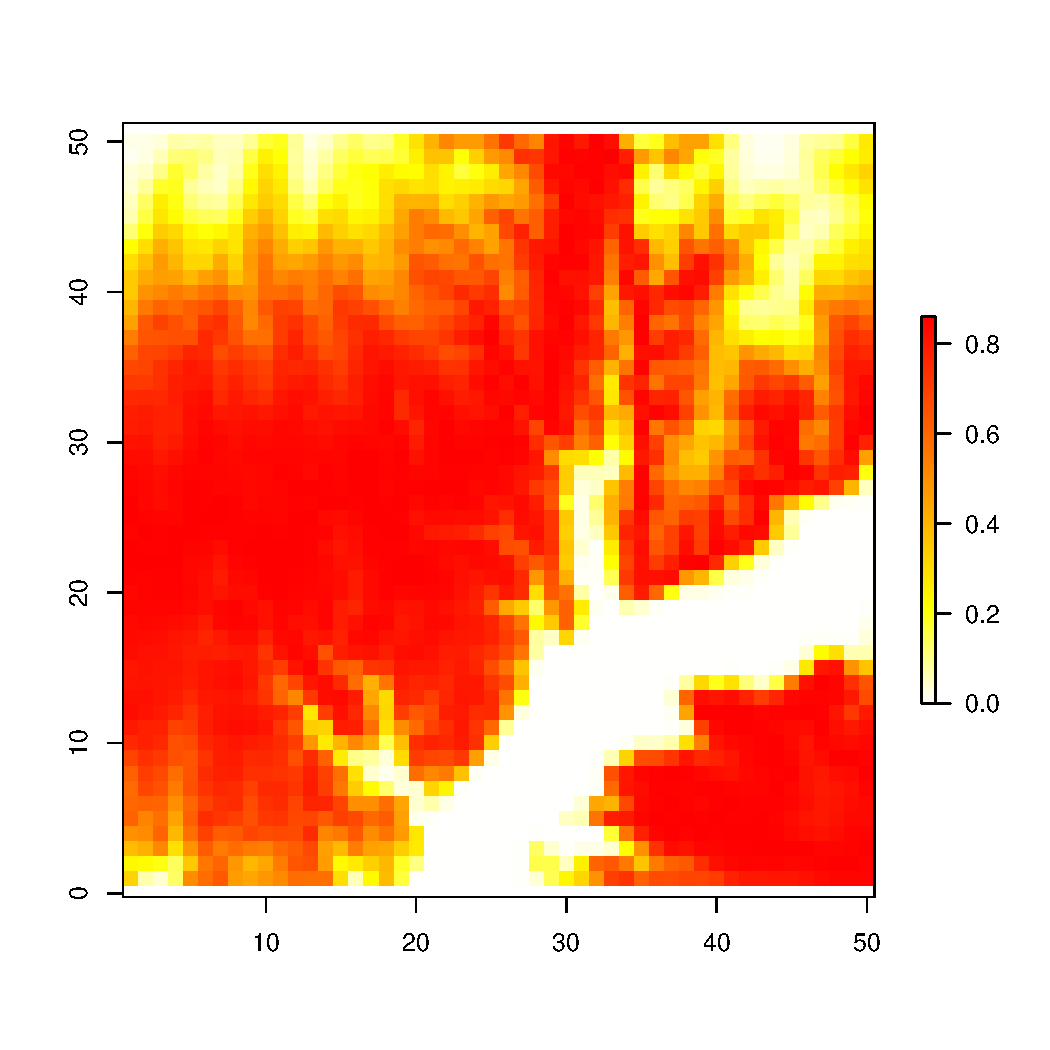
\includegraphics[width=8cm]{figures/predictions-binomial3.pdf} \\
  \end{tabular}
  
  \caption{\textbf{Predicted probability of presence and uncertainty of predictions}. Mean
    probability of presence (top), predictions at 2.5\% quantile (bottom left) and 97.5\%
    quantile (bottom right) can be plotted from the \texttt{mcmc} object
    \texttt{plot.p.pred} returned by function \texttt{hSDM.binomial()}.}
  
  \label{fig:predictions-binomial}
  
\end{figure}

In our example, we can compare the predictions to the initial probability of presence
computed from our model to check that our predictions are correct
(Fig.~\ref{fig:pred-obs-binomial}).

\begin{knitrout}\small
\definecolor{shadecolor}{rgb}{0.969, 0.969, 0.969}\color{fgcolor}\begin{kframe}
\begin{alltt}
\hlcom{# Comparing predictions to initial values}
\hlkwd{plot}\hlstd{(theta[],theta.pred.mean[],}\hlkwc{cex.lab}\hlstd{=}\hlnum{1.4}\hlstd{,}\hlkwc{xlim}\hlstd{=}\hlkwd{c}\hlstd{(}\hlnum{0}\hlstd{,}\hlnum{1}\hlstd{),}\hlkwc{ylim}\hlstd{=}\hlkwd{c}\hlstd{(}\hlnum{0}\hlstd{,}\hlnum{1}\hlstd{))}
\hlkwd{points}\hlstd{(theta[],theta.pred.2.5[],}\hlkwc{cex.lab}\hlstd{=}\hlnum{1.4}\hlstd{,}\hlkwc{col}\hlstd{=}\hlkwd{grey}\hlstd{(}\hlnum{0.5}\hlstd{))}
\hlkwd{points}\hlstd{(theta[],theta.pred.97.5[],}\hlkwc{cex.lab}\hlstd{=}\hlnum{1.4}\hlstd{,}\hlkwc{col}\hlstd{=}\hlkwd{grey}\hlstd{(}\hlnum{0.5}\hlstd{))}
\hlkwd{abline}\hlstd{(}\hlkwc{a}\hlstd{=}\hlnum{0}\hlstd{,}\hlkwc{b}\hlstd{=}\hlnum{1}\hlstd{,}\hlkwc{col}\hlstd{=}\hlstr{"red"}\hlstd{,}\hlkwc{lwd}\hlstd{=}\hlnum{2}\hlstd{)}
\end{alltt}
\end{kframe}
\end{knitrout}


\begin{figure} 
  \centering 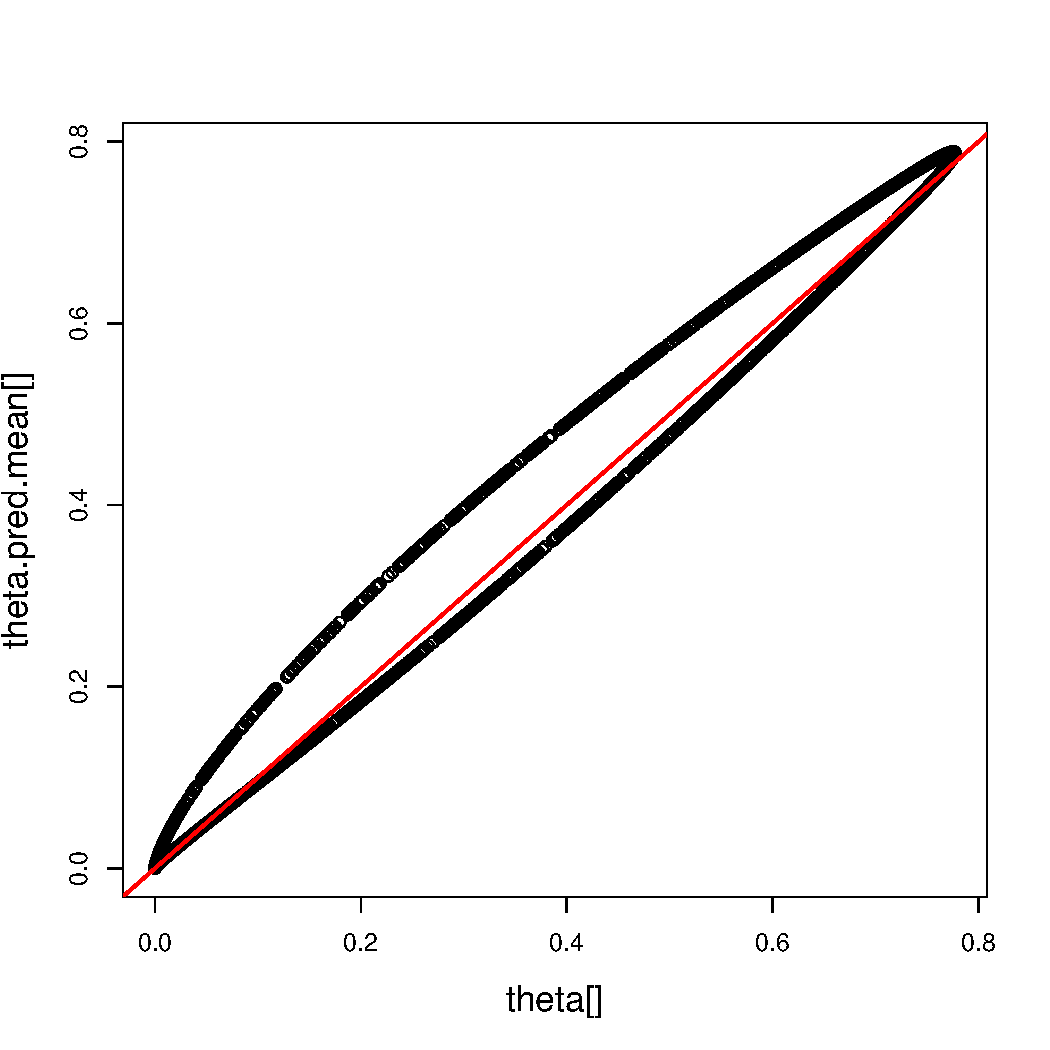
\includegraphics[width=8cm]{figures/pred-obs-binomial.pdf}
  
  \caption{\textbf{Predicted vs. initial probabilities of presence}. Initial probabilities
    of presence are computed from the Binomial logistic regression model with target
    parameters.}
  
  \label{fig:pred-obs-binomial}
  
\end{figure}

\newpage

\subsection{Site-occupancy model}

\subsubsection{Mathematical formulation}

Let's consider the random variable $z_i$ describing habitat suitability at site $i$. The
random variable $z_i$ can take value 1 or 0 depending on the fact that the habitat is
suitable ($z_i=1$) or not ($z_i=0$). Habitat at site $i$ is described by environmental
variables $X_i$. Random variable $z_i$ can be assumed to follow a Bernoulli distribution
of parameter $\theta_i$ (Eq.~\ref{eq:siteocc}). In this case, $\theta_i$ is the
probability that the habitat is suitable. Several visits at time $t_1$, $t_2$, etc., can
occur at site $i$. Let's consider the random variable $y_{it}$ representing the presence
of the species at site $i$ and time $t$. The species is observed at site $i$
($\sum_t{y_{it}} \geq 1$) only if the habitat is suitable ($z_i=1$). The species is
unobserved at site $i$ ($\sum_t{y_{it}}=0$) if the habitat is not suitable ($z_i=0$) or if
the habitat is suitable ($z_i=1$) but the probability $\delta_{it}$ of detecting the
species at site $i$ and time $t$ is inferior to 1. Thus, $y_{it}$ is assumed to follow a
Bernoulli distribution of parameter $z_i \delta_{it}$. Using a logit link function,
$\delta_{it}$ can be expressed as a linear model combining explicative variables $W_{it}$
and parameters $\gamma$ (Eq.~\ref{eq:siteocc}). Typically, explicative variables
$W_{it}$ are site characteristics (e.g., habitat variables) or survey characteristics
(e.g., weather conditions). The function \texttt{hSDM.siteocc()} estimates the parameters
$\beta$ and $\gamma$ of such a model.

\begin{equation}
  \begin{tabular}{c}
    \textbf{Ecological process:}\\
    $z_i \sim \mathcal{B}ernoulli(\theta_i)$ \\
    $\logit(\theta_i) = X_i \beta$\\
    ~ \\
    \textbf{Observation process:}\\
    $y_{it} \sim \mathcal{B}ernoulli(z_i \delta_{it})$ \\
    $\logit(\delta_{it}) = W_{it} \gamma$ \\
  \end{tabular}
  \label{eq:siteocc}
\end{equation}

\subsubsection{Data generation}

To explore the characteristics of the \texttt{hSDM.siteocc()} function, we can generate a
new virtual data-set on the basis of the site-occupancy model described above
(Eq.~\ref{eq:siteocc}). In the most general case, the observation protocol includes severals
visits with varying survey conditions (e.g. weather conditions) to several sites with
fixed sites characteristics (e.g. habitat variables). We will generate a virtual data-set
following this protocole using the altitudinal data in the previous example for the
Binomial model (Sec.~\ref{sec:binomial}).

We draw at random the number of visits at each site of the previous example (see
Fig.~\ref{fig:observations-binomial} of Sec.~\ref{sec:binomial}).

\begin{knitrout}\small
\definecolor{shadecolor}{rgb}{0.969, 0.969, 0.969}\color{fgcolor}\begin{kframe}
\begin{alltt}
\hlcom{# Number of visits associated to each observation point}
\hlkwd{set.seed}\hlstd{(seed)}
\hlstd{visits} \hlkwb{<-} \hlkwd{rpois}\hlstd{(nsite,}\hlkwc{lambda}\hlstd{=}\hlnum{3}\hlstd{)} \hlcom{# Mean number of visits ~3}
\hlcom{# NB: Setting a too low mean number of visits per site (lambda < 3)}
\hlcom{# leads to inaccurate parameter estimates}
\hlstd{visits[visits}\hlopt{==}\hlnum{0}\hlstd{]} \hlkwb{<-} \hlnum{1} \hlcom{# Number of visits must be > 0}
\hlcom{# Vector of observation sites}
\hlstd{sites} \hlkwb{<-} \hlkwd{vector}\hlstd{()}
\hlkwa{for} \hlstd{(i} \hlkwa{in} \hlnum{1}\hlopt{:}\hlstd{nsite) \{}
    \hlstd{sites} \hlkwb{<-} \hlkwd{c}\hlstd{(sites,}\hlkwd{rep}\hlstd{(i,visits[i]))}
\hlstd{\}}
\end{alltt}
\end{kframe}
\end{knitrout}


The survey conditions for each visit are determined by two explicative variables, $w_1$
and the altitude (variable denoted $A$). These two variables explain the observability of
the species (Eq.~\ref{eq:siteocc-detection}).

\begin{equation}
  \begin{tabular}{c}
    $y_{it} \sim \mathcal{B}ernoulli(z_i \delta_{it})$ \\
    $\logit(\delta_{it}) = \gamma_0 + \gamma_1 w_{1it} + \gamma_2 A_{it}$ \\
  \end{tabular}
  \label{eq:siteocc-detection}
\end{equation}

We fix the intercept and the effects of these two variables: $\gamma_0=-1$, $\gamma_1=1$
and $\gamma_2=-1$ for determining the detection probability. In our case, the detection
probability decreases with altitude ($\gamma_2 < 0$).

\begin{knitrout}\small
\definecolor{shadecolor}{rgb}{0.969, 0.969, 0.969}\color{fgcolor}\begin{kframe}
\begin{alltt}
\hlcom{# Explicative variables for observation process}
\hlstd{nobs} \hlkwb{<-} \hlkwd{sum}\hlstd{(visits)}
\hlkwd{set.seed}\hlstd{(seed)}
\hlstd{w1} \hlkwb{<-} \hlkwd{rnorm}\hlstd{(}\hlkwc{n}\hlstd{=nobs,}\hlnum{0}\hlstd{,}\hlnum{1}\hlstd{)}
\hlstd{W} \hlkwb{<-} \hlkwd{cbind}\hlstd{(}\hlkwd{rep}\hlstd{(}\hlnum{1}\hlstd{,nobs),w1,X.sites[sites,}\hlnum{2}\hlstd{])}
\hlcom{# Target parameters for observation process}
\hlstd{gamma.target} \hlkwb{<-} \hlkwd{matrix}\hlstd{(}\hlkwd{c}\hlstd{(}\hlopt{-}\hlnum{1}\hlstd{,}\hlnum{1}\hlstd{,}\hlopt{-}\hlnum{1}\hlstd{),}\hlkwc{ncol}\hlstd{=}\hlnum{1}\hlstd{)}
\end{alltt}
\end{kframe}
\end{knitrout}


Using covariates and parameters for the two processes, we compute the probability that
the habitat is suitable ($\theta_i$) and the species detection probability
($\delta_i$). We also draw the random variables $z_i$ and $y_i$ and construct the
observation data-set.

\begin{knitrout}\small
\definecolor{shadecolor}{rgb}{0.969, 0.969, 0.969}\color{fgcolor}\begin{kframe}
\begin{alltt}
\hlcom{# Ecological process (suitability)}
\hlstd{logit.theta.site} \hlkwb{<-} \hlstd{X.sites} \hlopt \hlstd{beta.target}
\hlstd{theta.site} \hlkwb{<-} \hlkwd{inv.logit}\hlstd{(logit.theta.site)}
\hlkwd{set.seed}\hlstd{(seed)}
\hlstd{Z} \hlkwb{<-} \hlkwd{rbinom}\hlstd{(nsite,}\hlnum{1}\hlstd{,theta.site)}

\hlcom{# Observation process (detectability)}
\hlstd{logit.delta.obs} \hlkwb{<-} \hlstd{W} \hlopt \hlstd{gamma.target}
\hlstd{delta.obs} \hlkwb{<-} \hlkwd{inv.logit}\hlstd{(logit.delta.obs)}
\hlkwd{set.seed}\hlstd{(seed)}
\hlstd{Y} \hlkwb{<-} \hlkwd{rbinom}\hlstd{(nobs,}\hlnum{1}\hlstd{,delta.obs}\hlopt{*}\hlstd{Z[sites])}

\hlcom{# Data-sets}
\hlstd{data.obs} \hlkwb{<-} \hlkwd{data.frame}\hlstd{(Y,w1,}\hlkwc{alt}\hlstd{=X.sites[sites,}\hlnum{2}\hlstd{],}\hlkwc{site}\hlstd{=sites)}
\hlstd{data.suit} \hlkwb{<-} \hlkwd{data.frame}\hlstd{(}\hlkwc{alt}\hlstd{=X.sites[,}\hlnum{2}\hlstd{])}
\end{alltt}
\end{kframe}
\end{knitrout}

\subsubsection{Parameter inference using the \texttt{hSDM.siteocc()} function}

The \texttt{hSDM.siteocc()} function estimates the parameter of a site-occupancy model in
a Bayesian framework.

\begin{knitrout}\small
\definecolor{shadecolor}{rgb}{0.969, 0.969, 0.969}\color{fgcolor}\begin{kframe}
\begin{alltt}
\hlstd{mod.hSDM.siteocc} \hlkwb{<-} \hlkwd{hSDM.siteocc}\hlstd{(}\hlcom{# Observations}
                                 \hlkwc{presence}\hlstd{=data.obs}\hlopt{$}\hlstd{Y,}
                                 \hlkwc{observability}\hlstd{=}\hlopt{~}\hlstd{w1}\hlopt{+}\hlstd{alt,}
                                 \hlkwc{site}\hlstd{=data.obs}\hlopt{$}\hlstd{site,}
                                 \hlkwc{data.observability}\hlstd{=data.obs,}
                                 \hlcom{# Habitat                                 }
                                 \hlkwc{suitability}\hlstd{=}\hlopt{~}\hlstd{alt,}
                                 \hlkwc{data.suitability}\hlstd{=data.suit,}
                                 \hlcom{# Predictions}
                                 \hlkwc{suitability.pred}\hlstd{=data.pred,}
                                 \hlcom{# Chains}
                                 \hlkwc{burnin}\hlstd{=}\hlnum{1000}\hlstd{,} \hlkwc{mcmc}\hlstd{=}\hlnum{1000}\hlstd{,} \hlkwc{thin}\hlstd{=}\hlnum{1}\hlstd{,}
                                 \hlcom{# Starting values}
                                 \hlkwc{beta.start}\hlstd{=}\hlnum{0}\hlstd{,}
                                 \hlkwc{gamma.start}\hlstd{=}\hlnum{0}\hlstd{,}
                                 \hlcom{# Priors}
                                 \hlkwc{mubeta}\hlstd{=}\hlnum{0}\hlstd{,} \hlkwc{Vbeta}\hlstd{=}\hlnum{1.0E6}\hlstd{,}
                                 \hlkwc{mugamma}\hlstd{=}\hlnum{0}\hlstd{,} \hlkwc{Vgamma}\hlstd{=}\hlnum{1.0E6}\hlstd{,}
                                 \hlcom{# Various}
                                 \hlkwc{seed}\hlstd{=}\hlnum{1234}\hlstd{,} \hlkwc{verbose}\hlstd{=}\hlnum{1}\hlstd{,} \hlkwc{save.p}\hlstd{=}\hlnum{1}\hlstd{)}
\end{alltt}
\end{kframe}
\end{knitrout}


\subsubsection{Analysis of the results}

\begin{knitrout}\small
\definecolor{shadecolor}{rgb}{0.969, 0.969, 0.969}\color{fgcolor}\begin{kframe}
\begin{alltt}
\hlkwd{summary}\hlstd{(mod.hSDM.siteocc}\hlopt{$}\hlstd{mcmc)}
\end{alltt}
\begin{verbatim}
## 
## Iterations = 1001:2000
## Thinning interval = 1 
## Number of chains = 1 
## Sample size per chain = 1000 
## 
## 1. Empirical mean and standard deviation for each variable,
##    plus standard error of the mean:
## 
##                      Mean    SD Naive SE Time-series SE
## beta.(Intercept)   -0.826 0.327  0.01035         0.0282
## beta.alt            1.110 0.445  0.01406         0.0341
## gamma.(Intercept)  -1.287 0.221  0.00698         0.0229
## gamma.w1            0.941 0.208  0.00658         0.0205
## gamma.alt          -0.930 0.220  0.00695         0.0200
## Deviance          295.730 3.092  0.09779         0.2765
## 
## 2. Quantiles for each variable:
## 
##                      2.5%     25%     50%     75%   97.5%
## beta.(Intercept)   -1.500  -1.041  -0.850  -0.586  -0.191
## beta.alt            0.417   0.738   1.031   1.445   2.077
## gamma.(Intercept)  -1.775  -1.438  -1.264  -1.142  -0.864
## gamma.w1            0.517   0.781   0.925   1.066   1.392
## gamma.alt          -1.398  -1.067  -0.924  -0.806  -0.504
## Deviance          291.769 293.442 295.091 297.205 304.031
\end{verbatim}
\end{kframe}
\end{knitrout}


\begin{knitrout}\small
\definecolor{shadecolor}{rgb}{0.969, 0.969, 0.969}\color{fgcolor}\begin{kframe}
\begin{alltt}
\hlkwd{plot}\hlstd{(mod.hSDM.siteocc}\hlopt{$}\hlstd{mcmc)}
\end{alltt}
\end{kframe}
\end{knitrout}


\begin{figure} 
  \begin{center}
    \begin{tabular}{cc}
      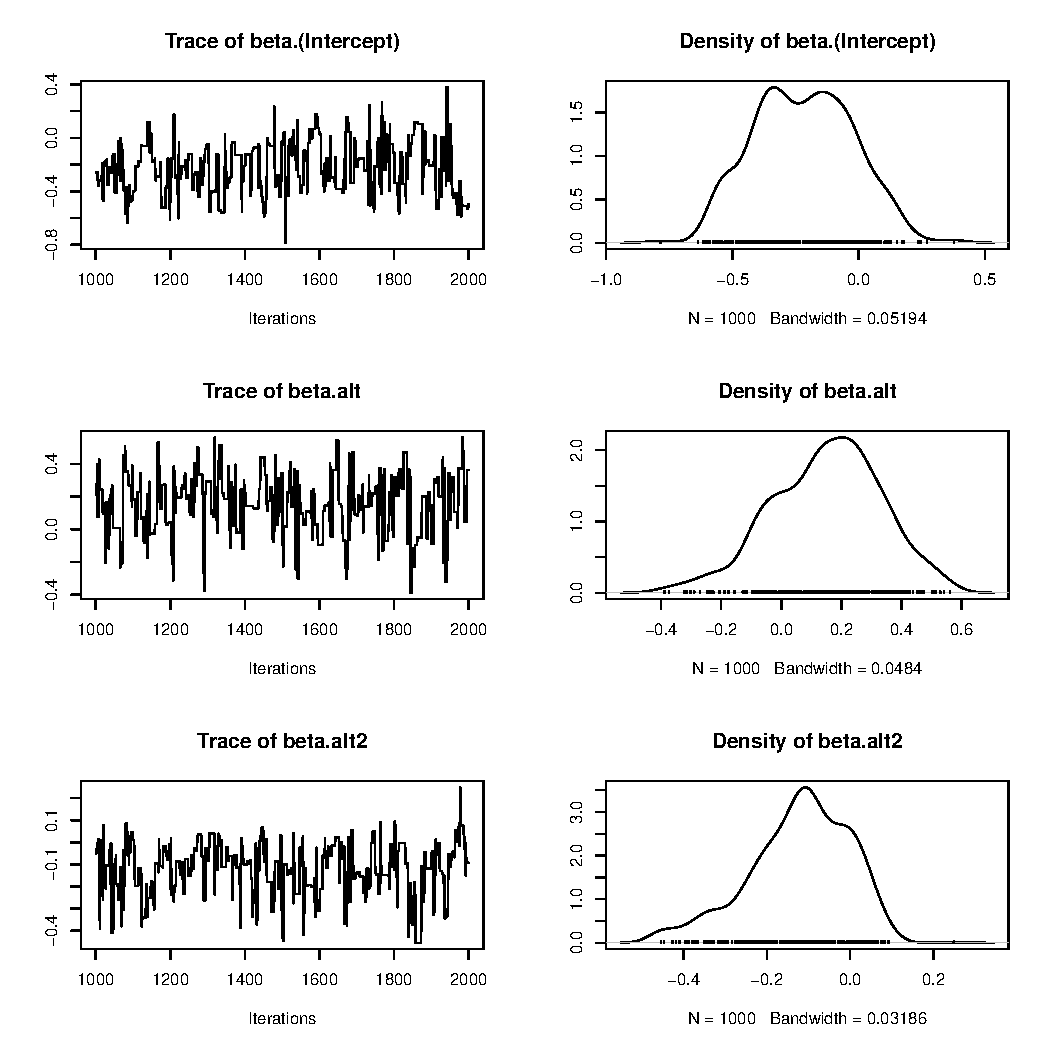
\includegraphics[width=8cm]{figures/mcmc-siteocc1.pdf} &
      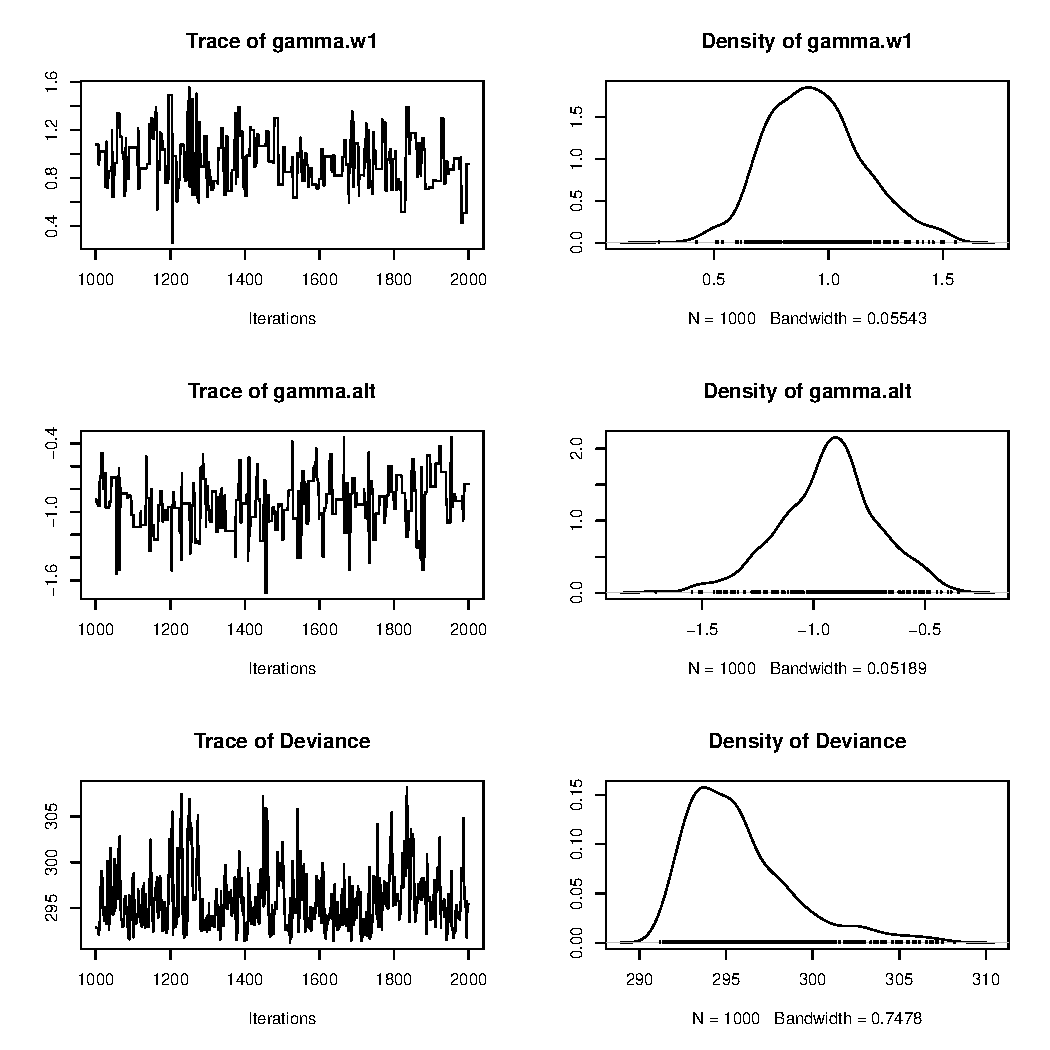
\includegraphics[width=8cm]{figures/mcmc-siteocc2.pdf} \\
    \end{tabular}
  \end{center}
  \caption{\textbf{Trace and density estimate for each variable of the MCMC}.}
  \label{fig:mcmc-siteocc}
\end{figure}

\begin{knitrout}\small
\definecolor{shadecolor}{rgb}{0.969, 0.969, 0.969}\color{fgcolor}\begin{kframe}
\begin{alltt}
\hlcom{# Create a raster for predictions}
\hlstd{theta.pred.mean} \hlkwb{<-} \hlkwd{raster}\hlstd{(theta)}
\hlcom{# Computing mean and quantiles for uncertainty}
\hlstd{theta.pred.mean[]} \hlkwb{<-} \hlkwd{apply}\hlstd{(mod.hSDM.siteocc}\hlopt{$}\hlstd{theta.pred,}\hlnum{2}\hlstd{,mean)}
\hlstd{theta.pred.2.5} \hlkwb{<-} \hlkwd{apply}\hlstd{(mod.hSDM.siteocc}\hlopt{$}\hlstd{theta.pred,}\hlnum{2}\hlstd{,quantile,}\hlnum{0.025}\hlstd{)}
\hlstd{theta.pred.97.5} \hlkwb{<-} \hlkwd{apply}\hlstd{(mod.hSDM.siteocc}\hlopt{$}\hlstd{theta.pred,}\hlnum{2}\hlstd{,quantile,}\hlnum{0.975}\hlstd{)}
\hlcom{# Plot the predicted probability of presence}
\hlkwd{plot}\hlstd{(theta.pred.mean,}\hlkwc{main}\hlstd{=}\hlstr{"hSDM.siteocc"}\hlstd{,}\hlkwc{col}\hlstd{=}\hlkwd{colRP}\hlstd{(nb),}\hlkwc{breaks}\hlstd{=brks,}
     \hlkwc{axis.args}\hlstd{=arg,}\hlkwc{zlim}\hlstd{=}\hlkwd{c}\hlstd{(}\hlnum{0}\hlstd{,}\hlnum{1}\hlstd{))}
\end{alltt}
\end{kframe}
\end{knitrout}


\begin{knitrout}\small
\definecolor{shadecolor}{rgb}{0.969, 0.969, 0.969}\color{fgcolor}\begin{kframe}
\begin{alltt}
\hlcom{# Comparing predictions to initial values}
\hlkwd{plot}\hlstd{(theta[],theta.pred.mean[],}\hlkwc{xlim}\hlstd{=}\hlkwd{c}\hlstd{(}\hlnum{0}\hlstd{,}\hlnum{1}\hlstd{),}\hlkwc{ylim}\hlstd{=}\hlkwd{c}\hlstd{(}\hlnum{0}\hlstd{,}\hlnum{1}\hlstd{),}\hlkwc{cex.lab}\hlstd{=}\hlnum{1.4}\hlstd{)}
\hlkwd{points}\hlstd{(theta[],theta.pred.2.5[],}\hlkwc{cex.lab}\hlstd{=}\hlnum{1.4}\hlstd{,}\hlkwc{col}\hlstd{=}\hlkwd{grey}\hlstd{(}\hlnum{0.5}\hlstd{))}
\hlkwd{points}\hlstd{(theta[],theta.pred.97.5[],}\hlkwc{cex.lab}\hlstd{=}\hlnum{1.4}\hlstd{,}\hlkwc{col}\hlstd{=}\hlkwd{grey}\hlstd{(}\hlnum{0.5}\hlstd{))}
\hlkwd{abline}\hlstd{(}\hlkwc{a}\hlstd{=}\hlnum{0}\hlstd{,}\hlkwc{b}\hlstd{=}\hlnum{1}\hlstd{,}\hlkwc{col}\hlstd{=}\hlstr{"red"}\hlstd{,}\hlkwc{lwd}\hlstd{=}\hlnum{2}\hlstd{)}
\end{alltt}
\end{kframe}
\end{knitrout}



\begin{figure} 
  \begin{tabular}{cc}
    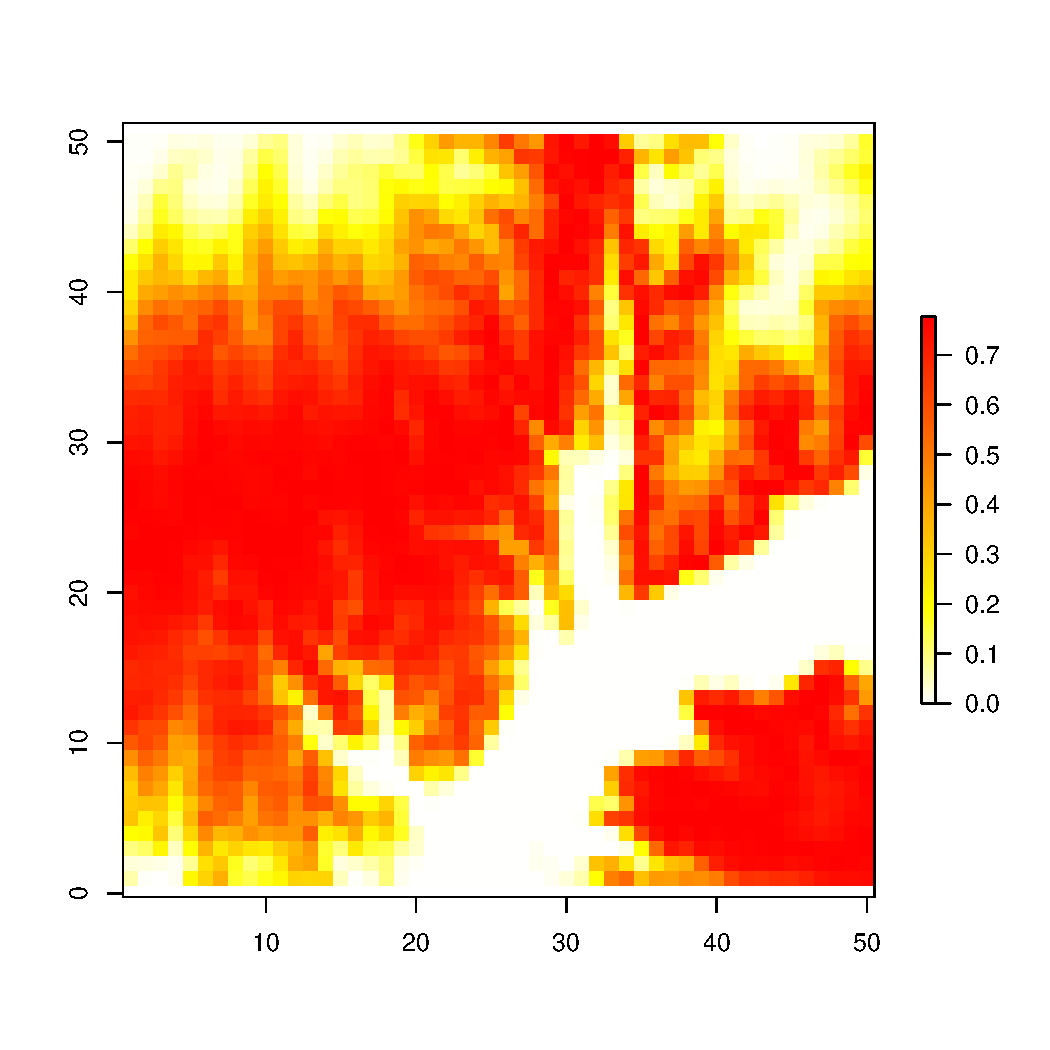
\includegraphics[width=8cm]{figures/theta-binomial.pdf} &
    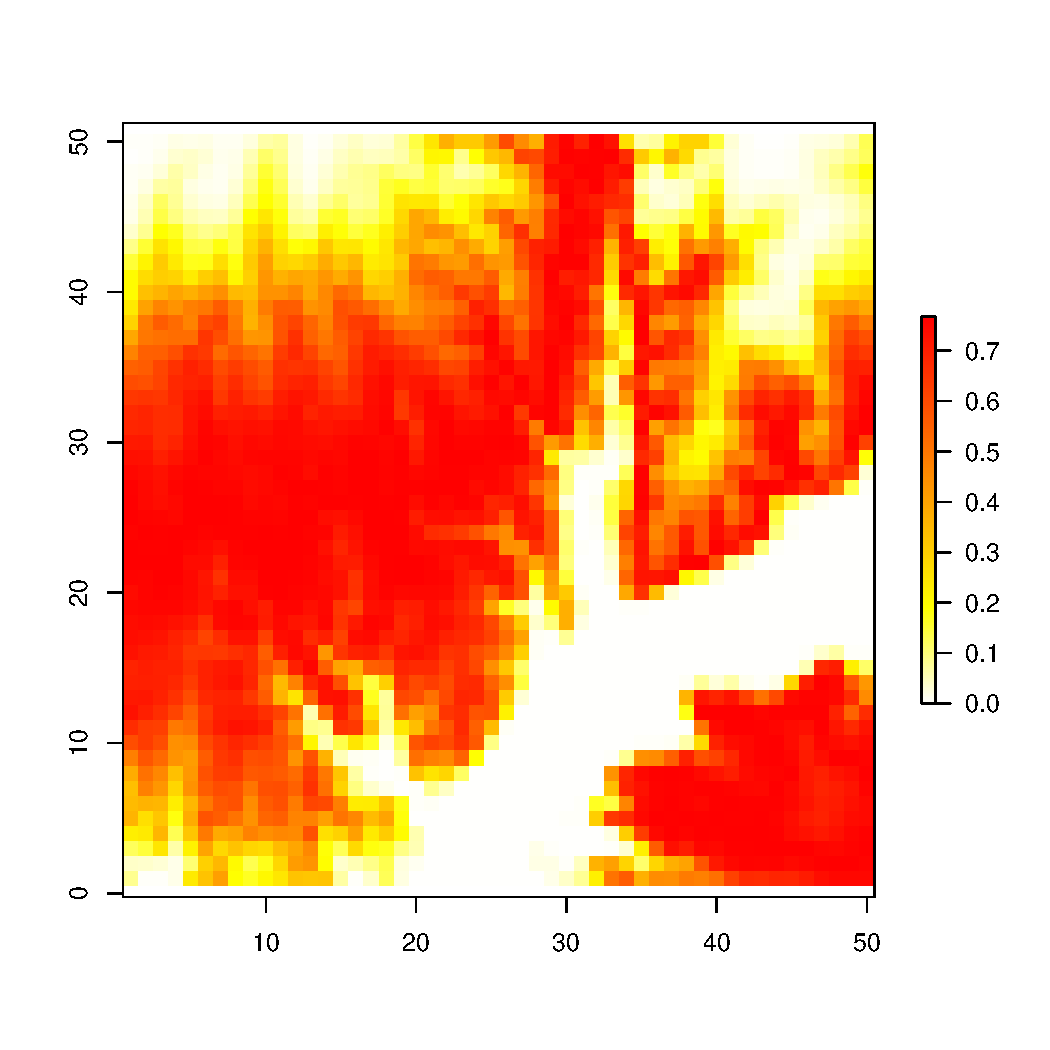
\includegraphics[width=8cm]{figures/predictions-siteocc.pdf} \\
  \end{tabular}
  \centering 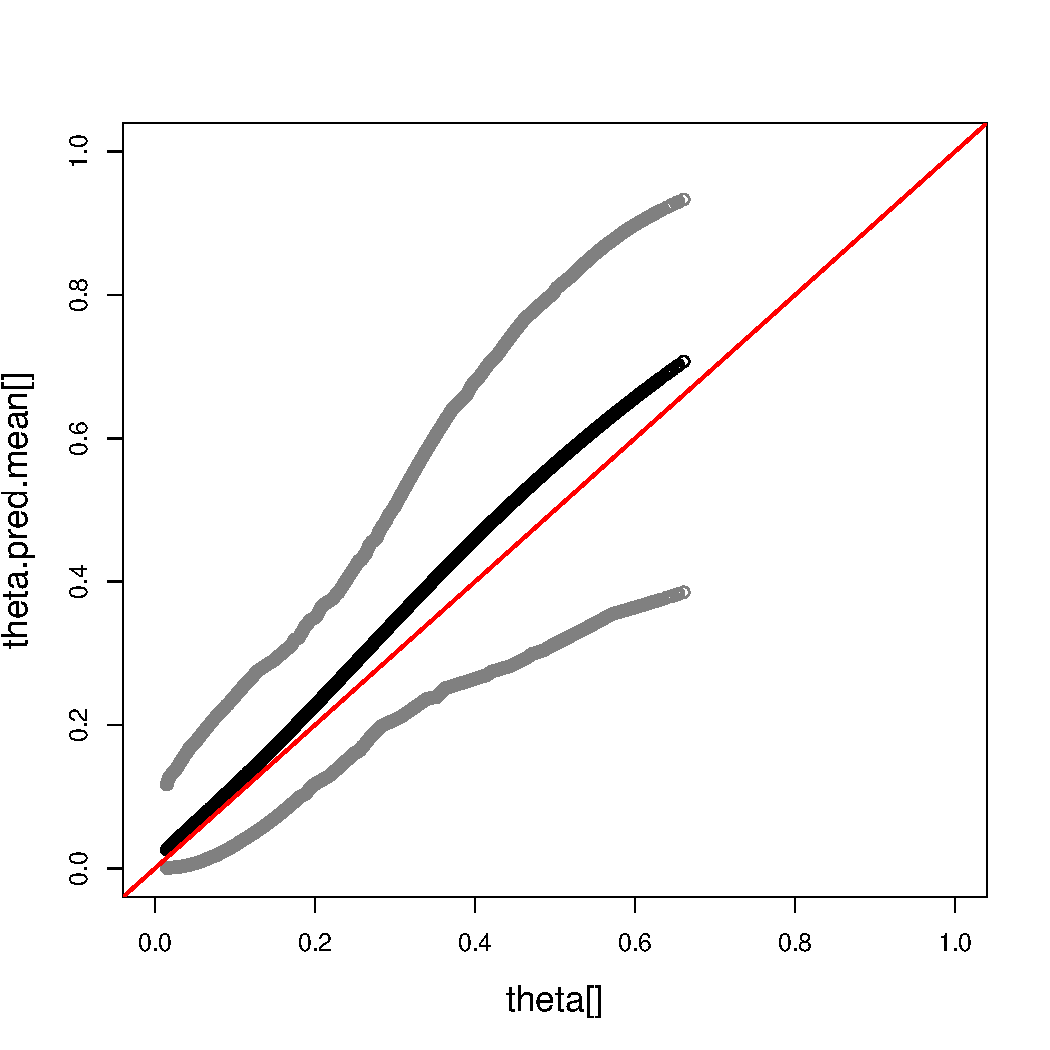
\includegraphics[width=8cm]{figures/pred-obs-siteocc.pdf} \\
  
  \caption{\textbf{Comparing predicted probability of presence with initial
      probabilities.}}
  
  \label{fig:predictions-siteocc}
  
\end{figure}

Parameters estimates can be compared to results obtained with the \texttt{glm()} function
assuming a perfect detection.

\begin{knitrout}\small
\definecolor{shadecolor}{rgb}{0.969, 0.969, 0.969}\color{fgcolor}\begin{kframe}
\begin{alltt}
\hlcom{#== glm results for comparison}
\hlstd{mod.glm} \hlkwb{<-} \hlkwd{glm}\hlstd{(Y}\hlopt{~}\hlstd{alt,}\hlkwc{family}\hlstd{=}\hlstr{"binomial"}\hlstd{,}\hlkwc{data}\hlstd{=data.obs)}
\hlkwd{summary}\hlstd{(mod.glm)}
\end{alltt}
\begin{verbatim}
## 
## Call:
## glm(formula = Y ~ alt, family = "binomial", data = data.obs)
## 
## Deviance Residuals: 
##    Min      1Q  Median      3Q     Max  
## -0.528  -0.442  -0.427  -0.408   2.265  
## 
## Coefficients:
##             Estimate Std. Error z value Pr(>|z|)    
## (Intercept)   -2.318      0.144  -16.06   <2e-16 ***
## alt           -0.133      0.129   -1.03      0.3    
## ---
## Signif. codes:  0 '***' 0.001 '**' 0.01 '*' 0.05 '.' 0.1 ' ' 1
## 
## (Dispersion parameter for binomial family taken to be 1)
## 
##     Null deviance: 362.10  on 594  degrees of freedom
## Residual deviance: 361.08  on 593  degrees of freedom
## AIC: 365.1
## 
## Number of Fisher Scoring iterations: 5
\end{verbatim}
\end{kframe}
\end{knitrout}


\begin{knitrout}\small
\definecolor{shadecolor}{rgb}{0.969, 0.969, 0.969}\color{fgcolor}\begin{kframe}
\begin{alltt}
\hlcom{# Create a raster for predictions}
\hlstd{theta.pred.glm} \hlkwb{<-} \hlkwd{raster}\hlstd{(theta)}
\hlcom{# Attribute predicted values to raster cells}
\hlstd{theta.pred.glm[]} \hlkwb{<-} \hlkwd{predict.glm}\hlstd{(mod.glm,}\hlkwc{newdata}\hlstd{=data.pred,}\hlkwc{type}\hlstd{=}\hlstr{"response"}\hlstd{)}
\hlcom{# Plot the predicted probability of presence}
\hlkwd{plot}\hlstd{(theta.pred.glm,}\hlkwc{main}\hlstd{=}\hlstr{"GLM"}\hlstd{,}\hlkwc{col}\hlstd{=}\hlkwd{colRP}\hlstd{(nb),}\hlkwc{breaks}\hlstd{=brks,}
     \hlkwc{axis.args}\hlstd{=arg,}\hlkwc{zlim}\hlstd{=}\hlkwd{c}\hlstd{(}\hlnum{0}\hlstd{,}\hlnum{1}\hlstd{))}
\end{alltt}
\end{kframe}
\end{knitrout}


\begin{knitrout}\small
\definecolor{shadecolor}{rgb}{0.969, 0.969, 0.969}\color{fgcolor}\begin{kframe}
\begin{alltt}
\hlcom{# Comparing predictions to initial values}
\hlkwd{plot}\hlstd{(theta[],theta.pred.glm[],}
     \hlkwc{xlim}\hlstd{=}\hlkwd{c}\hlstd{(}\hlnum{0}\hlstd{,}\hlnum{1}\hlstd{),}\hlkwc{ylim}\hlstd{=}\hlkwd{c}\hlstd{(}\hlnum{0}\hlstd{,}\hlnum{1}\hlstd{),}\hlkwc{cex.lab}\hlstd{=}\hlnum{1.4}\hlstd{)}
\hlkwd{points}\hlstd{(theta[],theta.pred.mean[],}\hlkwc{col}\hlstd{=}\hlkwd{grey}\hlstd{(}\hlnum{0.5}\hlstd{))}
\hlkwd{abline}\hlstd{(}\hlkwc{a}\hlstd{=}\hlnum{0}\hlstd{,}\hlkwc{b}\hlstd{=}\hlnum{1}\hlstd{,}\hlkwc{col}\hlstd{=}\hlstr{"red"}\hlstd{,}\hlkwc{lwd}\hlstd{=}\hlnum{2}\hlstd{)}
\end{alltt}
\end{kframe}
\end{knitrout}


On Figure \ref{fig:predictions-siteocc-glm}, we can see that using a GLM in the case of
imperfect detection can lead to very inaccurate parameter estimates and predictions for
the probability of presence of the species. This is particularly true when detection
probability is negatively correlated to presence probability (through an explicative
variable such as the altitude in our example). This has been clearly demonstrated in an
article by \citet{Lahoz-Monfort2014}.

\begin{figure} 
  \begin{tabular}{cc}
    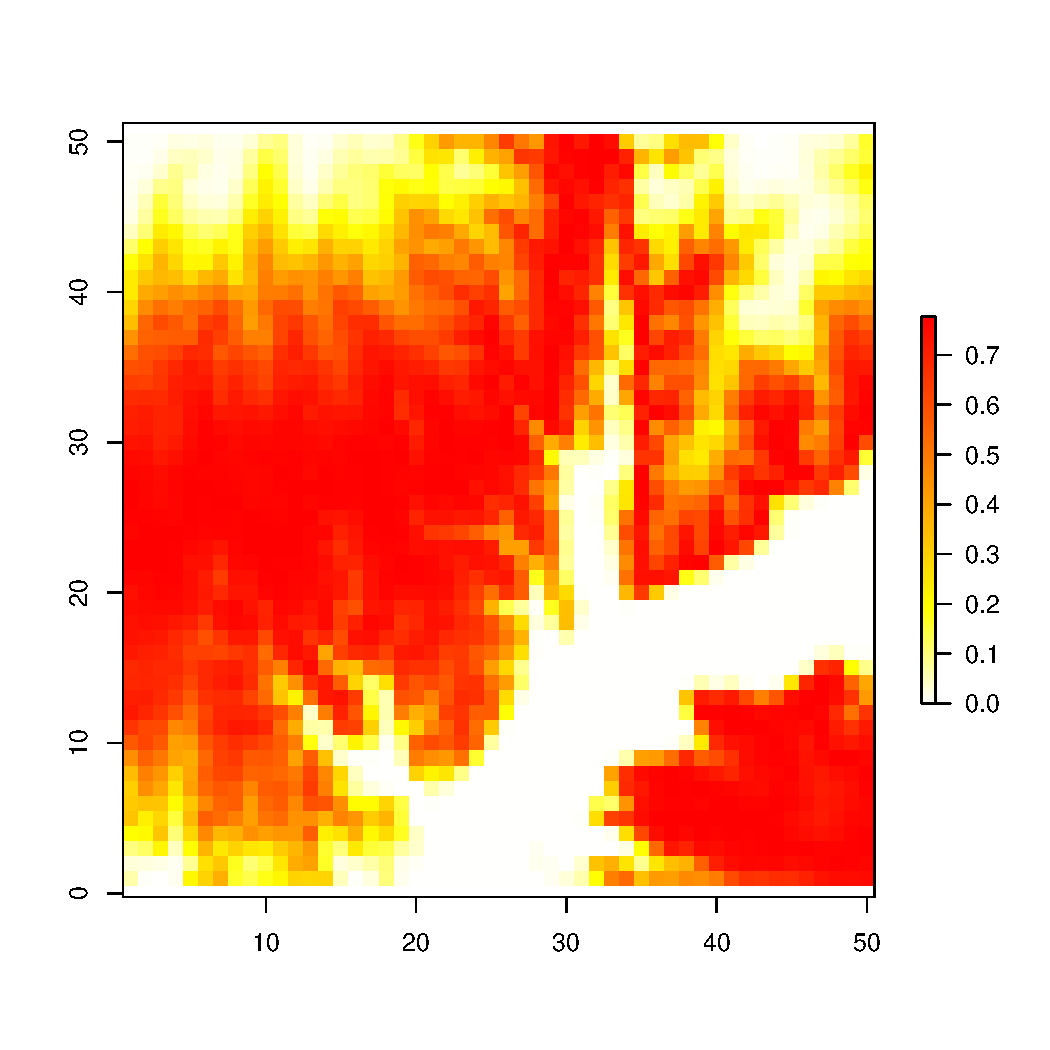
\includegraphics[width=8cm]{figures/theta-binomial.pdf} &
    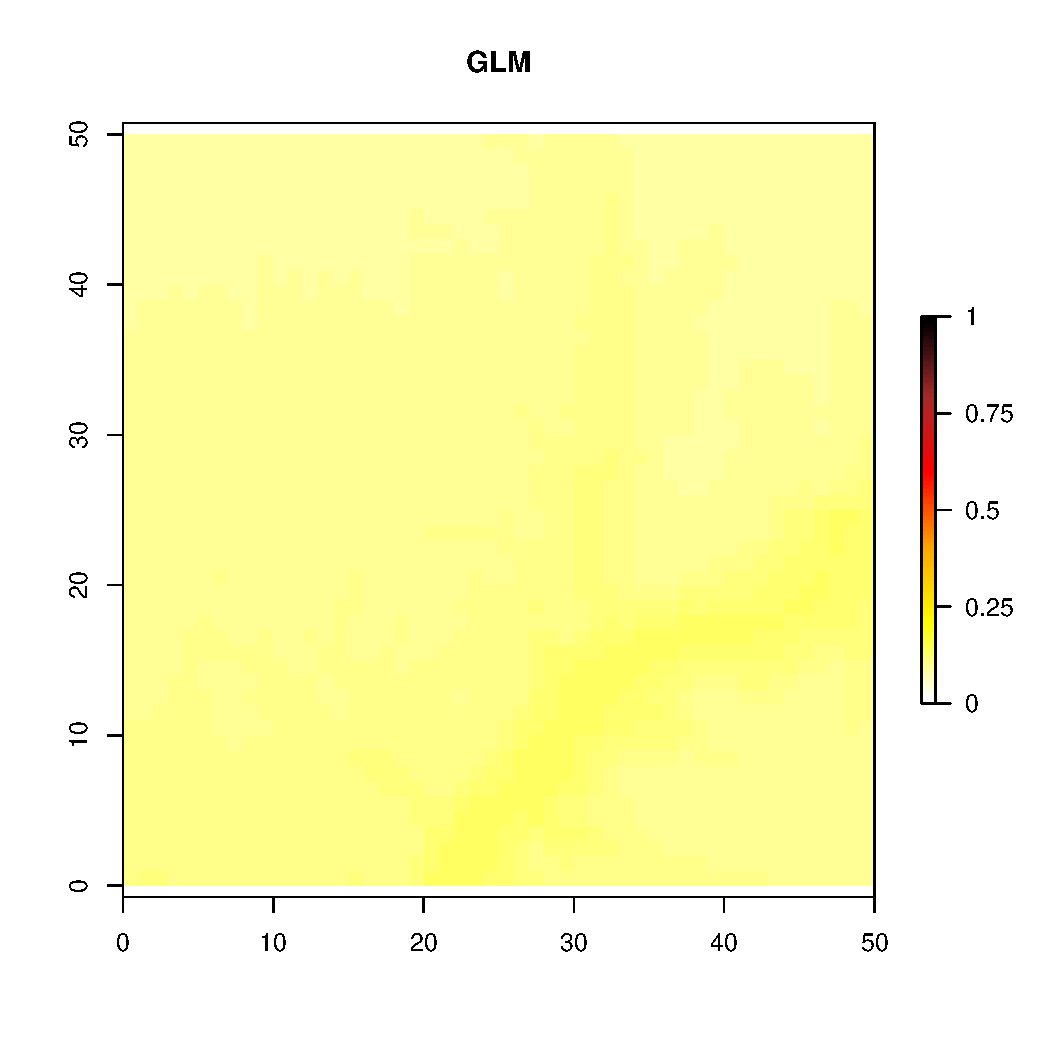
\includegraphics[width=8cm]{figures/predictions-siteocc-glm.pdf} \\
  \end{tabular}
  \centering 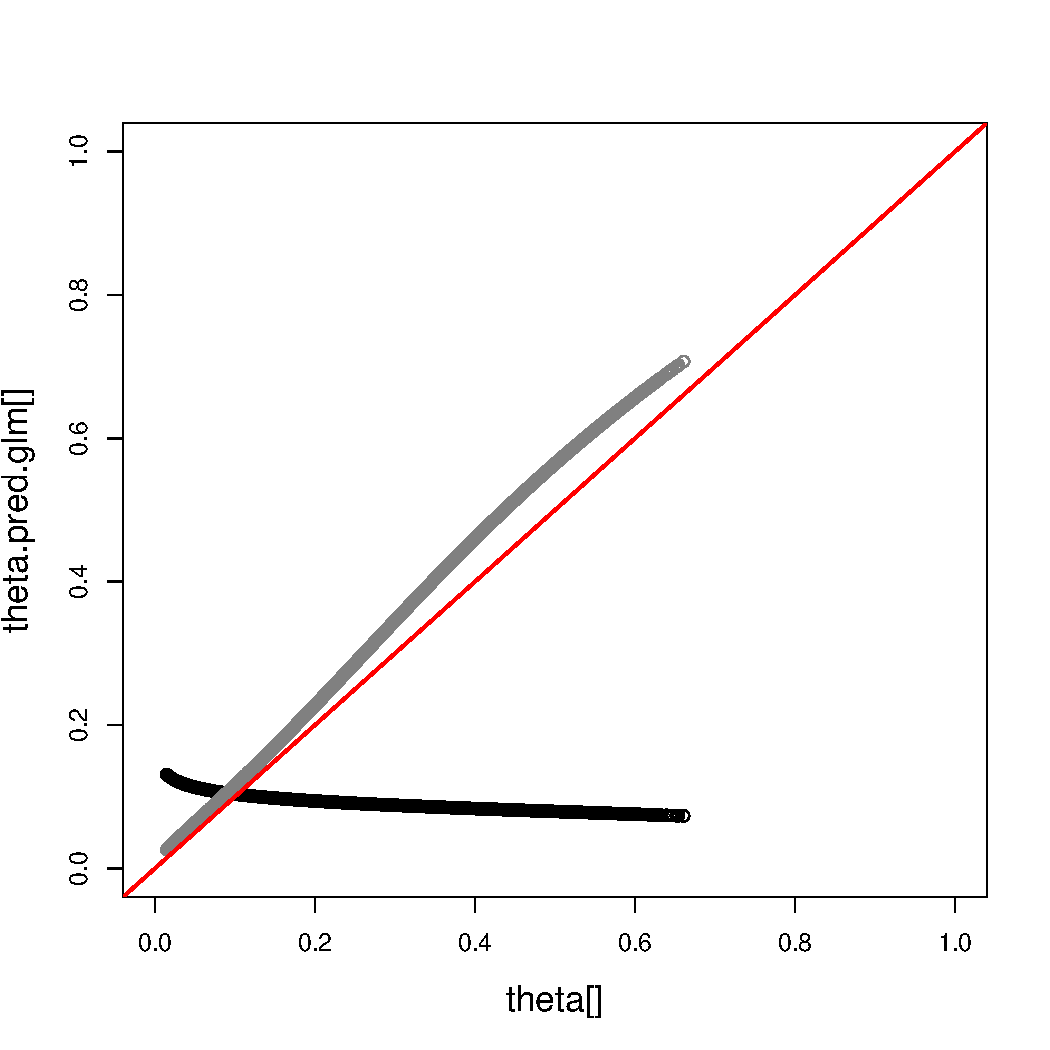
\includegraphics[width=8cm]{figures/pred-obs-siteocc-glm.pdf} \\
  
  \caption{\textbf{Comparing predicted probability of presence using GLM with initial
      probabilities.} Grey dots figure the predictions with the \texttt{hSDM.siteocc()}
    function whereas black dots figure the prediction using the \texttt{glm()} function.}
  
  \label{fig:predictions-siteocc-glm}
  
\end{figure}

\newpage

\subsection{Binomial iCAR model}

\subsubsection{Mathematical formulation}

\subsubsection{Data generation with iCAR}

\begin{knitrout}\small
\definecolor{shadecolor}{rgb}{0.969, 0.969, 0.969}\color{fgcolor}\begin{kframe}
\begin{alltt}
\hlcom{# Rasters must be projected to correctly compute the neighborhood}
\hlkwd{crs}\hlstd{(alt)} \hlkwb{<-} \hlstr{'+proj=utm +zone=1'}
\hlcom{# Neighborhood matrix}
\hlstd{neighbors.mat} \hlkwb{<-} \hlkwd{adjacent}\hlstd{(alt,} \hlkwc{cells}\hlstd{=}\hlkwd{c}\hlstd{(}\hlnum{1}\hlopt{:}\hlstd{ncells),} \hlkwc{directions}\hlstd{=}\hlnum{8}\hlstd{,}
                          \hlkwc{pairs}\hlstd{=}\hlnum{TRUE}\hlstd{,} \hlkwc{sorted}\hlstd{=}\hlnum{TRUE}\hlstd{)}
\hlcom{# Number of neighbors by cell}
\hlstd{n.neighbors} \hlkwb{<-} \hlkwd{as.data.frame}\hlstd{(}\hlkwd{table}\hlstd{(}\hlkwd{as.factor}\hlstd{(neighbors.mat[,}\hlnum{1}\hlstd{])))[,}\hlnum{2}\hlstd{]}
\hlcom{# Adjacent cells}
\hlstd{adj} \hlkwb{<-} \hlstd{neighbors.mat[,}\hlnum{2}\hlstd{]}
\hlcom{# Generate symmetric adjacency matrix, A}
\hlstd{A} \hlkwb{<-} \hlkwd{matrix}\hlstd{(}\hlnum{0}\hlstd{,ncells,ncells)}
\hlstd{index.start} \hlkwb{<-} \hlnum{1}
\hlkwa{for} \hlstd{(i} \hlkwa{in} \hlnum{1}\hlopt{:}\hlstd{ncells) \{}
    \hlstd{index.end} \hlkwb{<-} \hlstd{index.start}\hlopt{+}\hlstd{n.neighbors[i]}\hlopt{-}\hlnum{1}
    \hlstd{A[i,adj[}\hlkwd{c}\hlstd{(index.start}\hlopt{:}\hlstd{index.end)]]} \hlkwb{<-} \hlnum{1}
    \hlstd{index.start} \hlkwb{<-} \hlstd{index.end}\hlopt{+}\hlnum{1}
\hlstd{\}}
\end{alltt}
\end{kframe}
\end{knitrout}


\begin{knitrout}\small
\definecolor{shadecolor}{rgb}{0.969, 0.969, 0.969}\color{fgcolor}\begin{kframe}
\begin{alltt}
\hlcom{# Function to draw in a multivariate normal}
\hlstd{rmvn} \hlkwb{<-} \hlkwa{function}\hlstd{(}\hlkwc{n}\hlstd{,} \hlkwc{mu}\hlstd{=}\hlnum{0}\hlstd{,} \hlkwc{V}\hlstd{=}\hlkwd{matrix}\hlstd{(}\hlnum{1}\hlstd{),} \hlkwc{seed}\hlstd{=}\hlnum{1234}\hlstd{) \{}
    \hlstd{p} \hlkwb{<-} \hlkwd{length}\hlstd{(mu)}
    \hlkwa{if} \hlstd{(}\hlkwd{any}\hlstd{(}\hlkwd{is.na}\hlstd{(}\hlkwd{match}\hlstd{(}\hlkwd{dim}\hlstd{(V), p)))) \{}
        \hlkwd{stop}\hlstd{(}\hlstr{"Dimension problem!"}\hlstd{)}
    \hlstd{\}}
    \hlstd{D} \hlkwb{<-} \hlkwd{chol}\hlstd{(V)}
    \hlkwd{set.seed}\hlstd{(seed)}
    \hlkwd{t}\hlstd{(}\hlkwd{matrix}\hlstd{(}\hlkwd{rnorm}\hlstd{(n}\hlopt{*}\hlstd{p),}\hlkwc{ncol}\hlstd{=p)}\hlopt\hlstd{D}\hlopt{+}\hlkwd{rep}\hlstd{(mu,}\hlkwd{rep}\hlstd{(n,p)))}
\hlstd{\}}
\end{alltt}
\end{kframe}
\end{knitrout}


\begin{knitrout}\small
\definecolor{shadecolor}{rgb}{0.969, 0.969, 0.969}\color{fgcolor}\begin{kframe}
\begin{alltt}
\hlcom{# Generate spatial random effects}
\hlstd{Vrho.target} \hlkwb{<-} \hlnum{1} \hlcom{# Variance of spatial random effects}
\hlstd{d} \hlkwb{<-} \hlnum{1}  \hlcom{# Spatial dependence parameter = 1 for intrinsic CAR}
\hlstd{Q} \hlkwb{<-} \hlkwd{diag}\hlstd{(n.neighbors)}\hlopt{-}\hlstd{d}\hlopt{*}\hlstd{A} \hlopt{+} \hlkwd{diag}\hlstd{(}\hlnum{.0001}\hlstd{,ncells)} \hlcom{# Add small constant to }
                                               \hlcom{# make Q non-singular}
\hlstd{covrho} \hlkwb{<-} \hlstd{Vrho.target}\hlopt{*}\hlkwd{solve}\hlstd{(Q)} \hlcom{# Covariance of rhos}
\hlstd{rho} \hlkwb{<-} \hlkwd{c}\hlstd{(}\hlkwd{rmvn}\hlstd{(}\hlnum{1}\hlstd{,}\hlkwc{mu}\hlstd{=}\hlkwd{rep}\hlstd{(}\hlnum{0}\hlstd{,ncells),}\hlkwc{V}\hlstd{=covrho,}\hlkwc{seed}\hlstd{=seed))} \hlcom{# Spatial Random Effects}
\hlstd{rho} \hlkwb{<-} \hlstd{rho}\hlopt{-}\hlkwd{mean}\hlstd{(rho)} \hlcom{# Centering rhos on zero}
\hlstd{rho.rast} \hlkwb{<-} \hlkwd{rasterFromXYZ}\hlstd{(}\hlkwc{xyz}\hlstd{=}\hlkwd{cbind}\hlstd{(coords,rho))}
\hlcom{# Probability of presence}
\hlstd{theta.cells} \hlkwb{<-} \hlkwd{inv.logit}\hlstd{(X} \hlopt \hlstd{beta.target} \hlopt{+} \hlstd{rho)}
\hlstd{theta} \hlkwb{<-} \hlkwd{rasterFromXYZ}\hlstd{(}\hlkwd{cbind}\hlstd{(coords,theta.cells))}
\end{alltt}
\end{kframe}
\end{knitrout}


\begin{knitrout}\small
\definecolor{shadecolor}{rgb}{0.969, 0.969, 0.969}\color{fgcolor}\begin{kframe}
\begin{alltt}
\hlcom{# Ecological process (suitability)}
\hlstd{cells} \hlkwb{<-} \hlkwd{extract}\hlstd{(alt,sites.sp,}\hlkwc{cell}\hlstd{=}\hlnum{TRUE}\hlstd{)[,}\hlnum{1}\hlstd{]}
\hlkwd{set.seed}\hlstd{(seed)}
\hlstd{logit.theta.site} \hlkwb{<-} \hlstd{X.sites} \hlopt \hlstd{beta.target} \hlopt{+} \hlstd{rho[cells]}
\hlstd{theta.site} \hlkwb{<-} \hlkwd{inv.logit}\hlstd{(logit.theta.site)}
\hlkwd{set.seed}\hlstd{(seed)}
\hlstd{Y} \hlkwb{<-} \hlkwd{rbinom}\hlstd{(nsite,visits,theta.site)}
\hlcom{# Data-sets}
\hlstd{data.suit} \hlkwb{<-} \hlkwd{data.frame}\hlstd{(Y,visits,}\hlkwc{alt}\hlstd{=X.sites[,}\hlnum{2}\hlstd{],cells)}
\hlstd{data.pred} \hlkwb{<-} \hlkwd{data.frame}\hlstd{(}\hlkwc{alt}\hlstd{=}\hlkwd{values}\hlstd{(alt),}\hlkwc{cells}\hlstd{=}\hlkwd{c}\hlstd{(}\hlnum{1}\hlopt{:}\hlstd{ncells))}
\hlcom{# Transform observations into a spatial object}
\hlstd{data.suit} \hlkwb{<-} \hlkwd{SpatialPointsDataFrame}\hlstd{(}\hlkwc{coords}\hlstd{=}\hlkwd{coordinates}\hlstd{(sites.sp),}
                                    \hlkwc{data}\hlstd{=data.suit)}
\end{alltt}
\end{kframe}
\end{knitrout}


\begin{knitrout}\small
\definecolor{shadecolor}{rgb}{0.969, 0.969, 0.969}\color{fgcolor}\begin{kframe}
\begin{alltt}
\hlcom{# Plot spatial random effects}
\hlkwd{plot}\hlstd{(rho.rast,}\hlkwc{main}\hlstd{=}\hlstr{"Spatial random effects"}\hlstd{)}
\hlcom{# Plot initial probabilities and observations}
\hlkwd{plot}\hlstd{(theta,}\hlkwc{main}\hlstd{=}\hlstr{"Initial probabilities (iCAR model)"}\hlstd{,}\hlkwc{col}\hlstd{=}\hlkwd{colRP}\hlstd{(nb),}\hlkwc{breaks}\hlstd{=brks,}
     \hlkwc{axis.args}\hlstd{=arg,}\hlkwc{zlim}\hlstd{=}\hlkwd{c}\hlstd{(}\hlnum{0}\hlstd{,}\hlnum{1}\hlstd{))}
\hlkwd{points}\hlstd{(data.suit[data.suit}\hlopt{$}\hlstd{Y}\hlopt{>}\hlnum{0}\hlstd{,],}\hlkwc{pch}\hlstd{=}\hlnum{16}\hlstd{)}
\hlkwd{points}\hlstd{(data.suit[data.suit}\hlopt{$}\hlstd{Y}\hlopt{==}\hlnum{0}\hlstd{,],}\hlkwc{pch}\hlstd{=}\hlnum{1}\hlstd{)}
\end{alltt}
\end{kframe}
\end{knitrout}


\begin{figure} 
  \centering 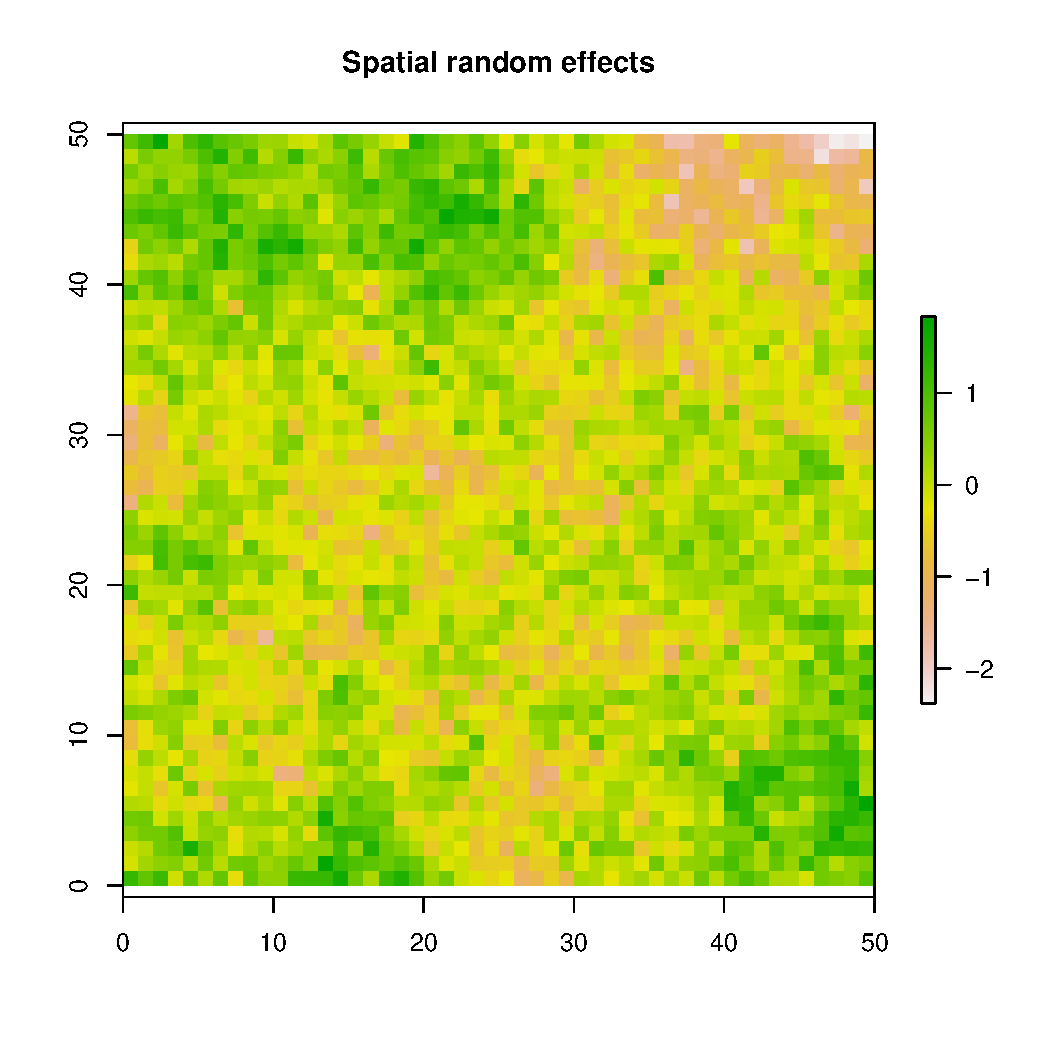
\includegraphics[width=8cm]{figures/binom-iCAR-plots1.pdf}
  \caption{\textbf{Spatial random effects.}}
  \label{fig:binom-iCAR-plots1-2}
\end{figure}

\begin{figure} 
  \centering 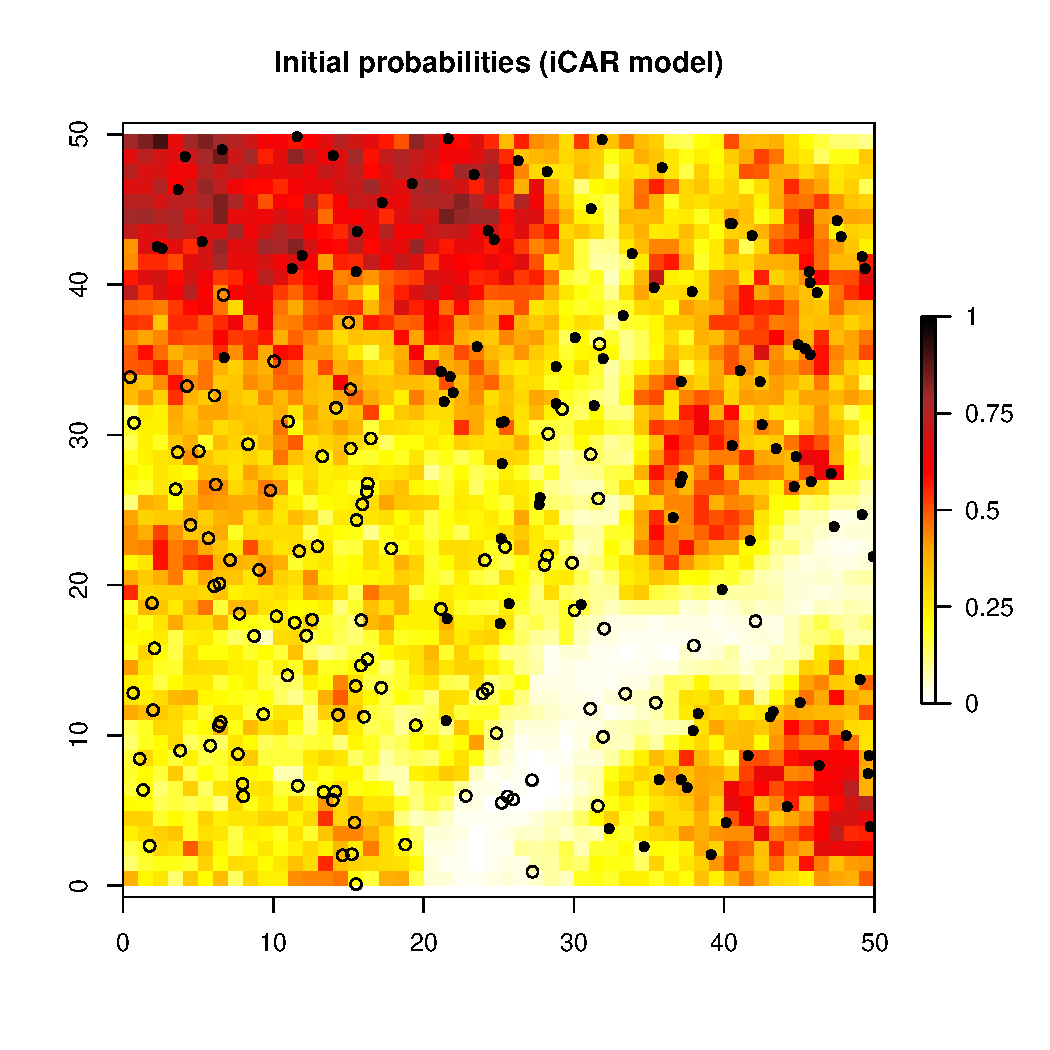
\includegraphics[width=8cm]{figures/binom-iCAR-plots2.pdf}
  \caption{\textbf{Initial probability of presence and observations.} 
    Presences (full circles) and absences (empty circles).}
  \label{fig:binom-iCAR-plots3}
\end{figure}

\subsubsection{Parameter inference using the \texttt{hSDM.binomial.iCAR()} function}

\begin{knitrout}\small
\definecolor{shadecolor}{rgb}{0.969, 0.969, 0.969}\color{fgcolor}\begin{kframe}
\begin{alltt}
\hlstd{Start} \hlkwb{<-} \hlkwd{Sys.time}\hlstd{()} \hlcom{# Start the clock}
\hlstd{mod.hSDM.binomial.iCAR} \hlkwb{<-} \hlkwd{hSDM.binomial.iCAR}\hlstd{(}\hlkwc{presences}\hlstd{=data.suit}\hlopt{$}\hlstd{Y,}
                                             \hlkwc{trials}\hlstd{=data.suit}\hlopt{$}\hlstd{visits,}
                                             \hlkwc{suitability}\hlstd{=}\hlopt{~}\hlstd{alt,}
                                             \hlkwc{spatial.entity}\hlstd{=data.suit}\hlopt{$}\hlstd{cells,}
                                             \hlkwc{data}\hlstd{=data.suit,}
                                             \hlkwc{n.neighbors}\hlstd{=n.neighbors,}
                                             \hlkwc{neighbors}\hlstd{=adj,}
                                             \hlkwc{suitability.pred}\hlstd{=data.pred,}
                                             \hlkwc{spatial.entity.pred}\hlstd{=data.pred}\hlopt{$}\hlstd{cells,}
                                             \hlkwc{burnin}\hlstd{=}\hlnum{5000}\hlstd{,} \hlkwc{mcmc}\hlstd{=}\hlnum{5000}\hlstd{,} \hlkwc{thin}\hlstd{=}\hlnum{5}\hlstd{,}
                                             \hlkwc{beta.start}\hlstd{=}\hlnum{0}\hlstd{,}
                                             \hlkwc{Vrho.start}\hlstd{=}\hlnum{1}\hlstd{,}
                                             \hlkwc{priorVrho}\hlstd{=}\hlstr{"1/Gamma"}\hlstd{,}
                                             \hlcom{#priorVrho="Uniform",}
                                             \hlcom{#priorVrho=1,}
                                             \hlkwc{mubeta}\hlstd{=}\hlnum{0}\hlstd{,} \hlkwc{Vbeta}\hlstd{=}\hlnum{1.0E6}\hlstd{,}
                                             \hlkwc{shape}\hlstd{=}\hlnum{0.5}\hlstd{,} \hlkwc{rate}\hlstd{=}\hlnum{0.0005}\hlstd{,}
                                             \hlkwc{Vrho.max}\hlstd{=}\hlnum{10}\hlstd{,}
                                             \hlkwc{seed}\hlstd{=}\hlnum{1234}\hlstd{,} \hlkwc{verbose}\hlstd{=}\hlnum{1}\hlstd{,}
                                             \hlkwc{save.rho}\hlstd{=}\hlnum{1}\hlstd{,} \hlkwc{save.p}\hlstd{=}\hlnum{0}\hlstd{)}
\hlstd{Time.hSDM} \hlkwb{<-} \hlkwd{difftime}\hlstd{(}\hlkwd{Sys.time}\hlstd{(),Start,}\hlkwc{units}\hlstd{=}\hlstr{"sec"}\hlstd{)} \hlcom{# Time difference}
\end{alltt}
\end{kframe}
\end{knitrout}


\subsubsection{Analysis of the results with iCAR}

\begin{knitrout}\small
\definecolor{shadecolor}{rgb}{0.969, 0.969, 0.969}\color{fgcolor}\begin{kframe}
\begin{alltt}
\hlkwd{summary}\hlstd{(mod.hSDM.binomial.iCAR}\hlopt{$}\hlstd{mcmc)}
\end{alltt}
\begin{verbatim}
## 
## Iterations = 5001:9996
## Thinning interval = 5 
## Number of chains = 1 
## Sample size per chain = 1000 
## 
## 1. Empirical mean and standard deviation for each variable,
##    plus standard error of the mean:
## 
##                    Mean     SD Naive SE Time-series SE
## beta.(Intercept)  -1.42  0.171  0.00542         0.0179
## beta.alt           1.14  0.221  0.00700         0.0318
## Vrho               3.24  0.932  0.02946         0.2401
## Deviance         259.97 10.747  0.33984         0.9438
## 
## 2. Quantiles for each variable:
## 
##                     2.5%    25%    50%    75%  97.5%
## beta.(Intercept)  -1.754  -1.53  -1.42  -1.30  -1.10
## beta.alt           0.734   1.00   1.14   1.28   1.63
## Vrho               1.930   2.56   3.05   3.78   5.55
## Deviance         241.580 252.20 259.24 267.29 281.26
\end{verbatim}
\end{kframe}
\end{knitrout}


\begin{knitrout}\small
\definecolor{shadecolor}{rgb}{0.969, 0.969, 0.969}\color{fgcolor}\begin{kframe}
\begin{alltt}
\hlcom{# Predictions for spatial random effects}
\hlstd{rho.pred} \hlkwb{<-} \hlkwd{apply}\hlstd{(mod.hSDM.binomial.iCAR}\hlopt{$}\hlstd{rho.pred,}\hlnum{2}\hlstd{,mean)}
\hlstd{rho.pred.rast} \hlkwb{<-} \hlkwd{rasterFromXYZ}\hlstd{(}\hlkwd{cbind}\hlstd{(coords,rho.pred))}
\hlkwd{plot}\hlstd{(rho.pred.rast,}\hlkwc{main}\hlstd{=}\hlstr{"Predictions rho"}\hlstd{)}
\hlcom{# Predictions for probability of presence}
\hlstd{theta.pred} \hlkwb{<-} \hlstd{mod.hSDM.binomial.iCAR}\hlopt{$}\hlstd{theta.pred}
\hlstd{theta.pred.rast} \hlkwb{<-} \hlkwd{rasterFromXYZ}\hlstd{(}\hlkwd{cbind}\hlstd{(coords,theta.pred))}
\hlkwd{plot}\hlstd{(theta.pred.rast,}\hlkwc{main}\hlstd{=}\hlstr{"Predictions theta"}\hlstd{,}\hlkwc{col}\hlstd{=}\hlkwd{colRP}\hlstd{(nb),}\hlkwc{breaks}\hlstd{=brks,}
     \hlkwc{axis.args}\hlstd{=arg,}\hlkwc{zlim}\hlstd{=}\hlkwd{c}\hlstd{(}\hlnum{0}\hlstd{,}\hlnum{1}\hlstd{))}
\hlcom{# Predictions vs. initial spatial random effects}
\hlkwd{plot}\hlstd{(rho[}\hlopt{-}\hlstd{cells],rho.pred[}\hlopt{-}\hlstd{cells],}\hlkwc{xlab}\hlstd{=}\hlstr{"rho target"}\hlstd{,}\hlkwc{ylab}\hlstd{=}\hlstr{"Predictions rho"}\hlstd{)}
\hlkwd{points}\hlstd{(rho[cells],rho.pred[cells],}\hlkwc{col}\hlstd{=}\hlstr{"blue"}\hlstd{,}\hlkwc{pch}\hlstd{=}\hlnum{16}\hlstd{)}
\hlkwd{abline}\hlstd{(}\hlkwc{a}\hlstd{=}\hlnum{0}\hlstd{,}\hlkwc{b}\hlstd{=}\hlnum{1}\hlstd{,}\hlkwc{col}\hlstd{=}\hlstr{"red"}\hlstd{)}
\hlcom{# Predictions vs. initial probabilities}
\hlkwd{plot}\hlstd{(}\hlkwd{values}\hlstd{(theta)[}\hlopt{-}\hlstd{cells],theta.pred[}\hlopt{-}\hlstd{cells],}\hlkwc{xlab}\hlstd{=}\hlstr{"theta target"}\hlstd{,}
     \hlkwc{ylab}\hlstd{=}\hlstr{"Predictions theta"}\hlstd{)}
\hlkwd{points}\hlstd{(}\hlkwd{values}\hlstd{(theta)[cells],theta.pred[cells],}\hlkwc{col}\hlstd{=}\hlstr{"blue"}\hlstd{,}\hlkwc{pch}\hlstd{=}\hlnum{16}\hlstd{)}
\hlkwd{abline}\hlstd{(}\hlkwc{a}\hlstd{=}\hlnum{0}\hlstd{,}\hlkwc{b}\hlstd{=}\hlnum{1}\hlstd{,}\hlkwc{col}\hlstd{=}\hlstr{"red"}\hlstd{)}
\end{alltt}
\end{kframe}
\end{knitrout}


\begin{figure}
  \begin{center}
    \begin{tabular}{cc}
      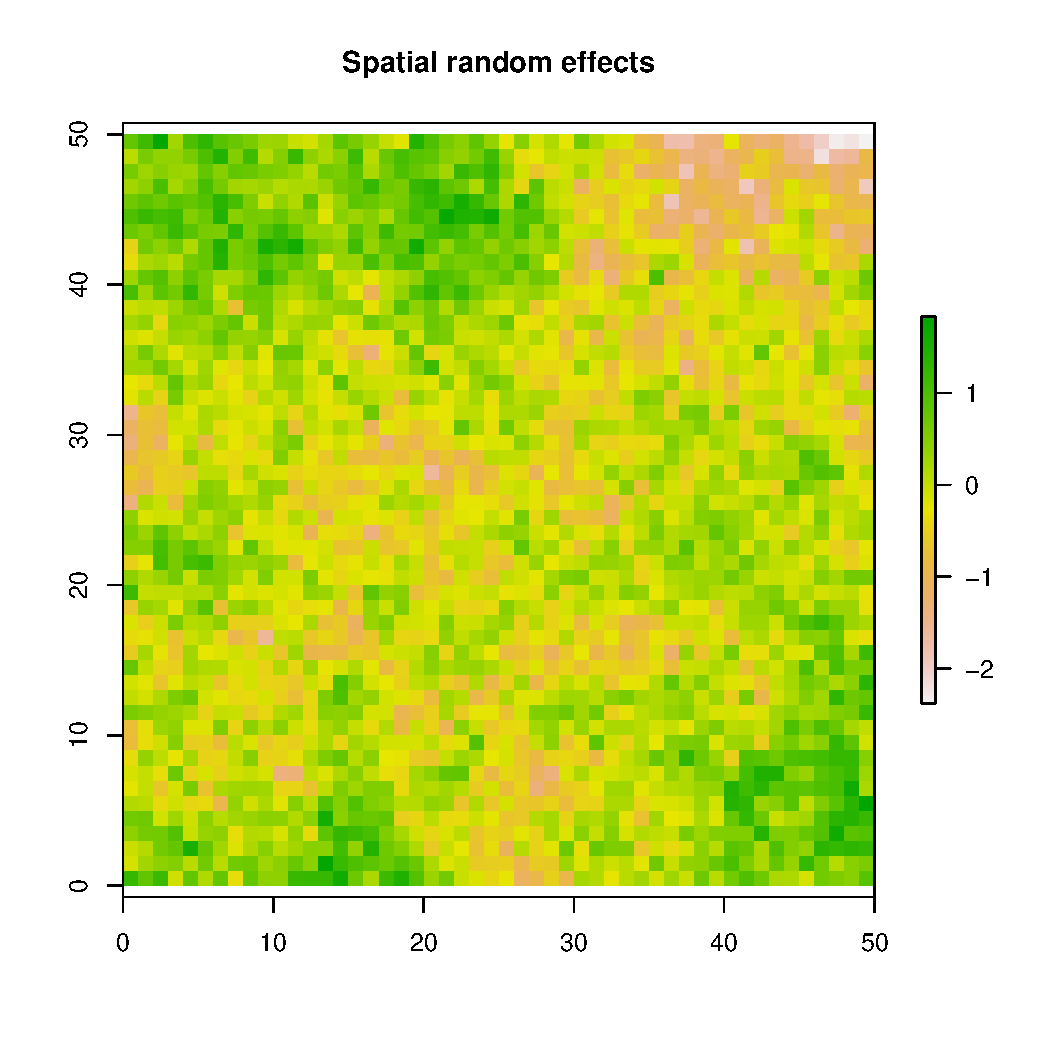
\includegraphics[width=6.5cm]{figures/binom-iCAR-plots1.pdf} & 
      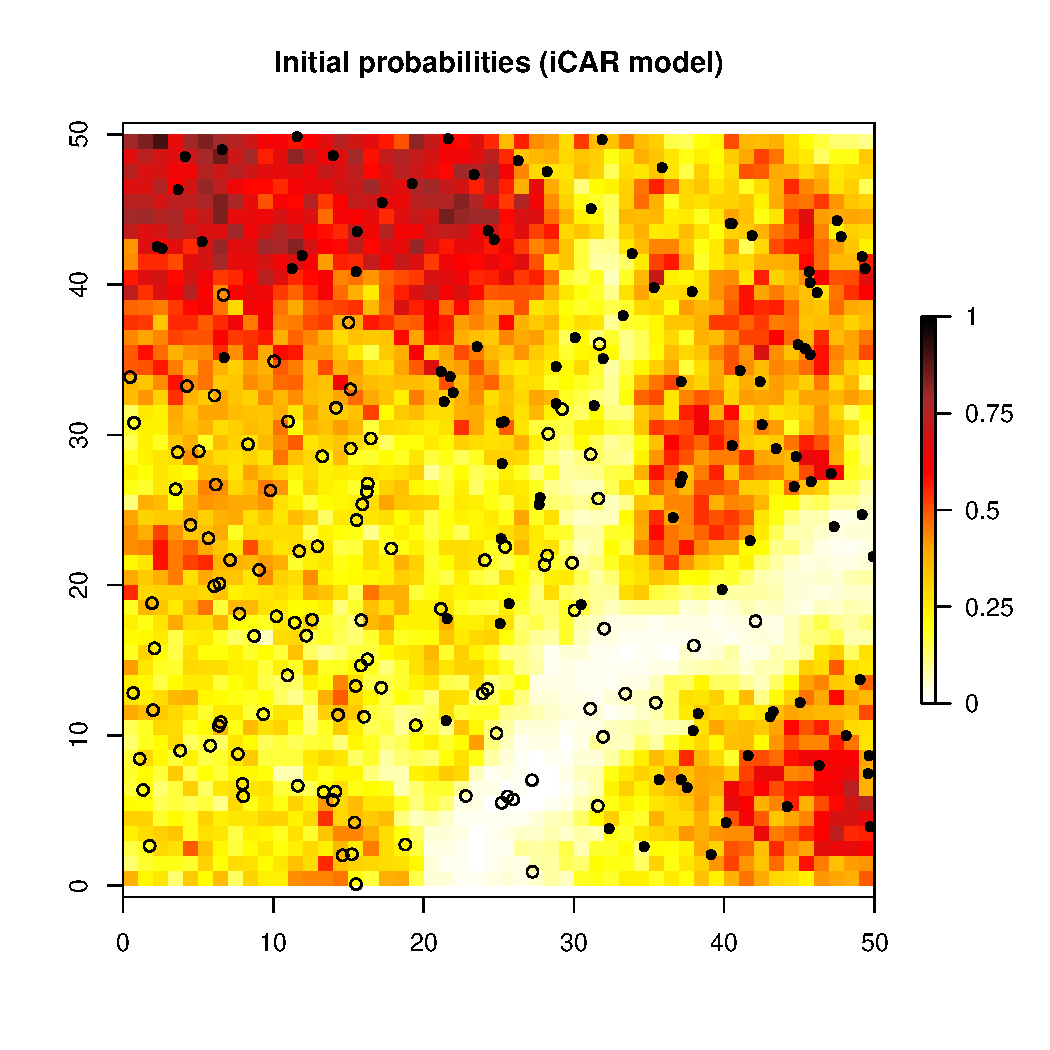
\includegraphics[width=6.5cm]{figures/binom-iCAR-plots2.pdf} \\
      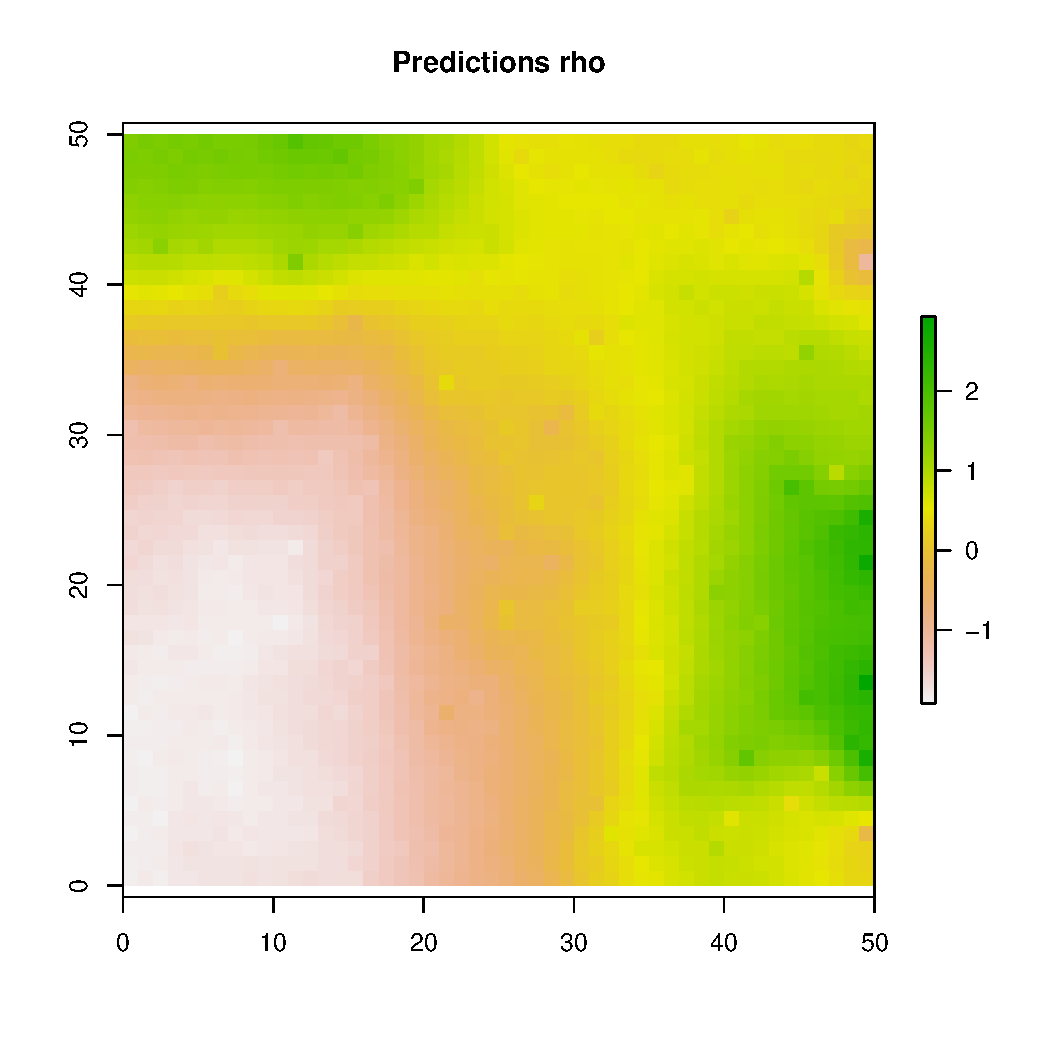
\includegraphics[width=6.5cm]{figures/binom-iCAR-results1.pdf} &
      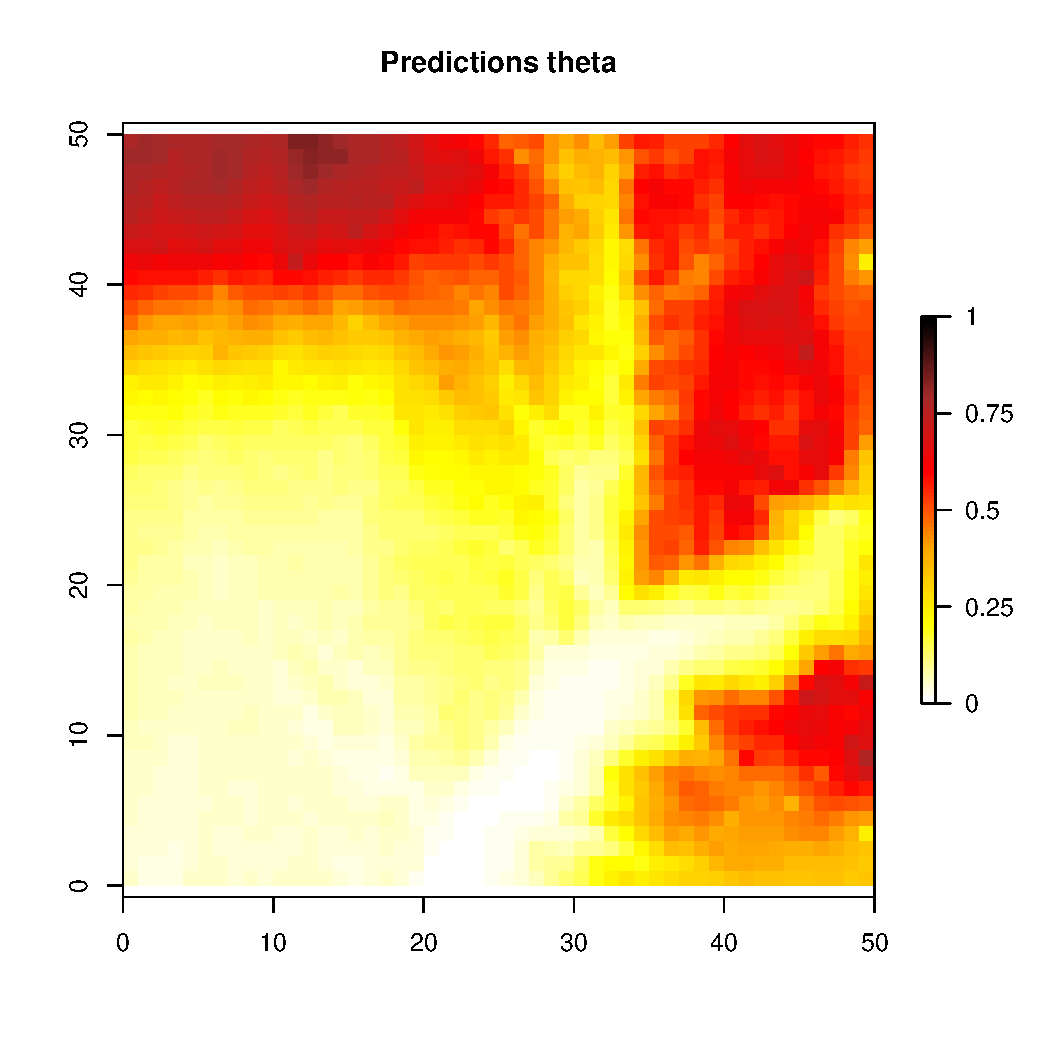
\includegraphics[width=6.5cm]{figures/binom-iCAR-results2.pdf} \\
      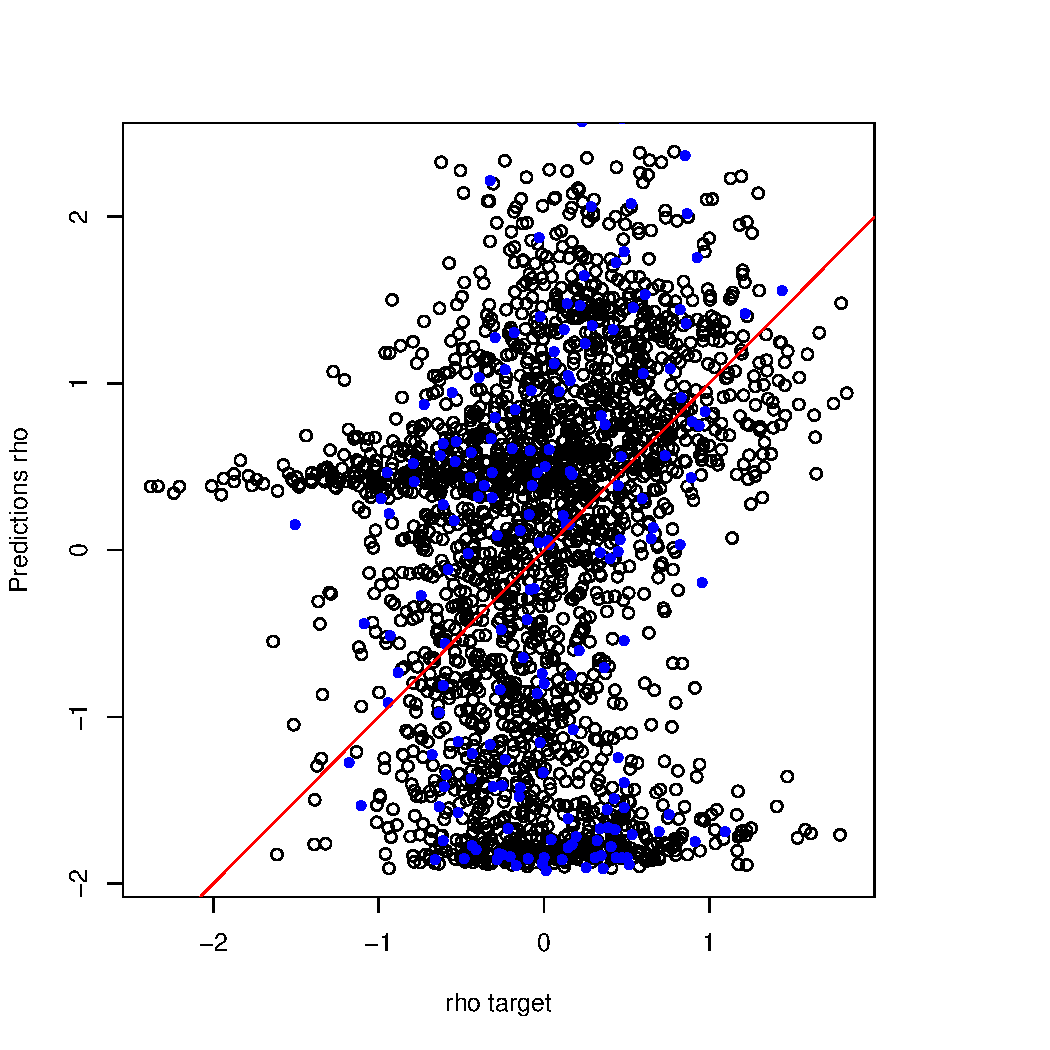
\includegraphics[width=6.5cm]{figures/binom-iCAR-results3.pdf} &
      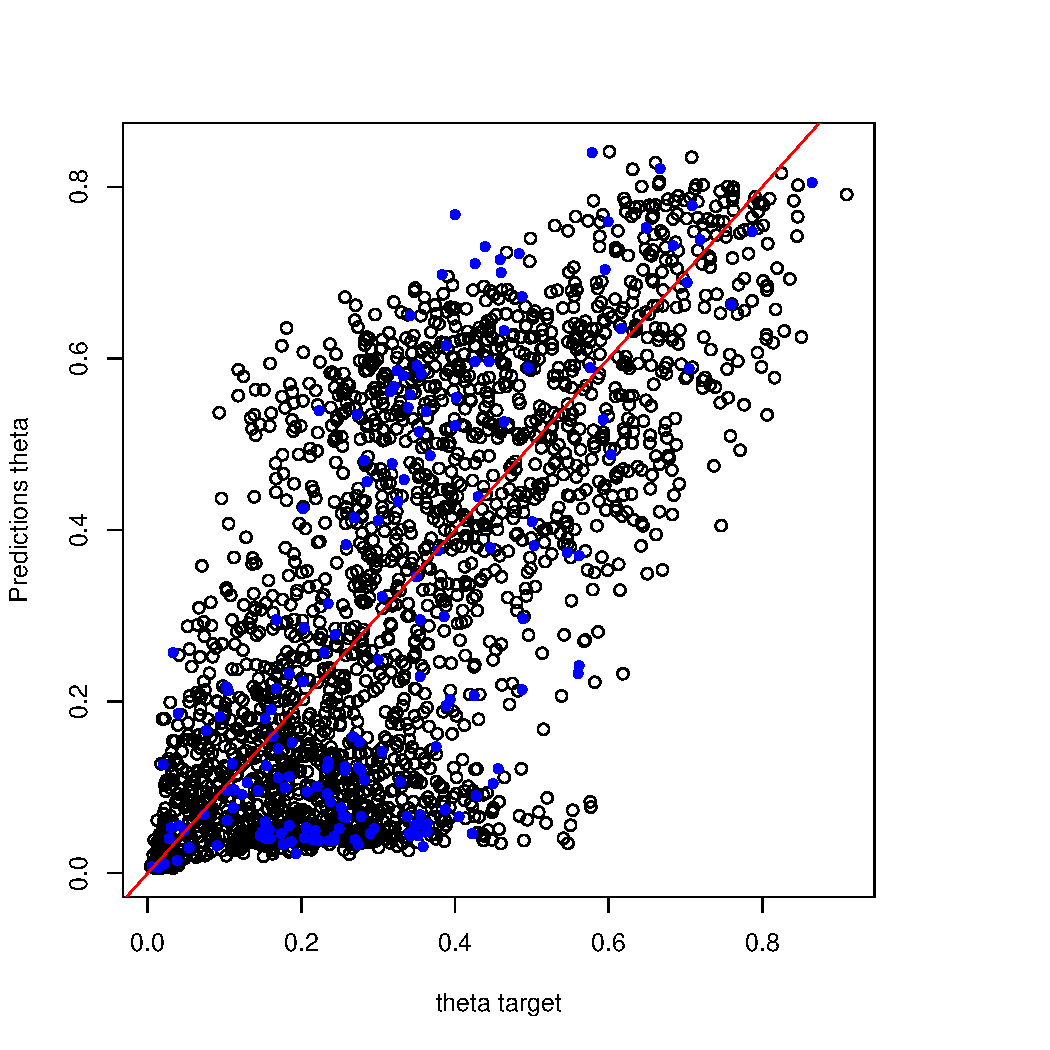
\includegraphics[width=6.5cm]{figures/binom-iCAR-results4.pdf} \\
    \end{tabular}
  \end{center}
  \caption{\textbf{Predictions vs. initial values}}
  \label{fig:binom-iCAR-results}
\end{figure}

\newpage

\subsubsection{With OpenBUGS}

\begin{knitrout}\small
\definecolor{shadecolor}{rgb}{0.969, 0.969, 0.969}\color{fgcolor}\begin{kframe}
\begin{alltt}
\hlcom{# BUGS model}
\hlstd{model.txt} \hlkwb{<-}
\hlstr{"model \{

# likelihood
for (n in 1:nobs) \{
  y[n] ~ dbin(theta[n], visits[n])
  logit(theta[n]) <- Xbeta[n] + rho[IdCell[n]]
  Xbeta[n] <- beta[1] + beta[2]*x1[n]
\}

# CAR prior distribution for spatial random effects:
rho[1:ncells] ~ car.normal(adj[], weights[], num[], tau)
for(k in 1:sumNumNeigh) \{
  weights[k] <- 1 # set equal weights for all neighbors
\}

# Other priors
for (i in 1:2) \{
  beta[i] ~ dnorm(0, 1.0E-6)
\}
Vrho <- 1/tau 
tau ~ dgamma(0.5,0.0005)

\}"}

\hlcom{# Create model.txt file in the working directory}
\hlkwd{system}\hlstd{(}\hlkwd{paste}\hlstd{(}\hlstr{"echo \textbackslash{}""}\hlstd{,model.txt,}\hlstr{"\textbackslash{}" > model.txt"}\hlstd{,}\hlkwc{sep}\hlstd{=}\hlstr{""}\hlstd{))}

\hlcom{# Data for OpenBUGS}
\hlstd{y} \hlkwb{<-} \hlstd{data.suit}\hlopt{$}\hlstd{Y}
\hlstd{visits} \hlkwb{<-} \hlstd{data.suit}\hlopt{$}\hlstd{visits}
\hlstd{IdCell} \hlkwb{<-} \hlstd{data.suit}\hlopt{$}\hlstd{cells}
\hlstd{x1} \hlkwb{<-} \hlstd{data.suit}\hlopt{$}\hlstd{alt}
\hlstd{num} \hlkwb{<-} \hlstd{n.neighbors}
\hlstd{adj} \hlkwb{<-} \hlstd{adj}
\hlstd{nobs} \hlkwb{<-} \hlkwd{length}\hlstd{(y)}
\hlstd{ncells} \hlkwb{<-} \hlkwd{length}\hlstd{(n.neighbors)}
\hlstd{sumNumNeigh} \hlkwb{<-} \hlkwd{length}\hlstd{(adj)}
\hlstd{data} \hlkwb{<-} \hlkwd{list}\hlstd{(}\hlstr{"y"}\hlstd{,}\hlstr{"visits"}\hlstd{,}\hlstr{"IdCell"}\hlstd{,}\hlstr{"x1"}\hlstd{,}\hlstr{"num"}\hlstd{,}
             \hlstr{"adj"}\hlstd{,}\hlstr{"nobs"}\hlstd{,}\hlstr{"ncells"}\hlstd{,}\hlstr{"sumNumNeigh"}\hlstd{)}

\hlcom{# Inits}
\hlstd{inits} \hlkwb{<-} \hlkwd{list}\hlstd{(}\hlkwd{list}\hlstd{(}\hlkwc{beta}\hlstd{=}\hlkwd{rep}\hlstd{(}\hlnum{0}\hlstd{,}\hlnum{2}\hlstd{),}\hlkwc{rho}\hlstd{=}\hlkwd{rep}\hlstd{(}\hlnum{0}\hlstd{,ncells),}\hlkwc{tau}\hlstd{=}\hlnum{1}\hlstd{))}

\hlcom{# OpenBUGS call}
\hlkwd{library}\hlstd{(R2OpenBUGS)}
\hlstd{Start} \hlkwb{<-} \hlkwd{Sys.time}\hlstd{()} \hlcom{# Start the clock}
\hlstd{Open} \hlkwb{<-} \hlkwd{bugs}\hlstd{(data,inits,}
             \hlkwc{model.file}\hlstd{=}\hlstr{"model.txt"}\hlstd{,}
             \hlkwc{parameters}\hlstd{=}\hlkwd{c}\hlstd{(}\hlstr{"beta"}\hlstd{,}\hlstr{"Vrho"}\hlstd{,}\hlstr{"rho"}\hlstd{),}
             \hlkwc{n.chains}\hlstd{=}\hlnum{1}\hlstd{,}
             \hlkwc{OpenBUGS.pgm}\hlstd{=}\hlstr{"/usr/local/bin/OpenBUGS"}\hlstd{,}
             \hlkwc{n.iter}\hlstd{=}\hlnum{2000}\hlstd{,}
             \hlkwc{n.burnin}\hlstd{=}\hlnum{1000}\hlstd{,}
             \hlkwc{n.thin}\hlstd{=}\hlnum{5}\hlstd{,}
             \hlkwc{DIC}\hlstd{=}\hlnum{TRUE}\hlstd{,}
             \hlkwc{debug}\hlstd{=}\hlnum{FALSE}\hlstd{,}
             \hlkwc{clearWD}\hlstd{=}\hlnum{FALSE}\hlstd{)}
\hlstd{Time.OpenBUGS} \hlkwb{<-} \hlkwd{difftime}\hlstd{(}\hlkwd{Sys.time}\hlstd{(),Start,}\hlkwc{units}\hlstd{=}\hlstr{"sec"}\hlstd{)} \hlcom{# Time difference}

\hlcom{# Time difference}
\hlstd{ratio.time} \hlkwb{<-} \hlkwd{as.numeric}\hlstd{(Time.OpenBUGS)}\hlopt{/}\hlkwd{as.numeric}\hlstd{(Time.hSDM)}
\hlstd{ratio.time} \hlcom{# For this example, hSDM is X times faster}

\hlcom{#== Outputs}
\hlkwd{attach.bugs}\hlstd{(Open,}\hlkwc{overwrite}\hlstd{=}\hlnum{TRUE}\hlstd{)}
\hlstd{Open}\hlopt{$}\hlstd{DIC}
\hlstd{Open}\hlopt{$}\hlstd{pD}
\hlstd{beta.pred.Open} \hlkwb{<-} \hlkwd{apply}\hlstd{(Open}\hlopt{$}\hlstd{sims.list}\hlopt{$}\hlstd{beta,}\hlnum{2}\hlstd{,mean)}
\hlstd{Vrho.pred.Open} \hlkwb{<-} \hlkwd{mean}\hlstd{(Open}\hlopt{$}\hlstd{sims.list}\hlopt{$}\hlstd{Vrho)}
\hlstd{deviance.Open} \hlkwb{<-} \hlkwd{mean}\hlstd{(Open}\hlopt{$}\hlstd{sims.list}\hlopt{$}\hlstd{deviance)}
\hlstd{rho.OpenBUGS} \hlkwb{<-} \hlkwd{apply}\hlstd{(Open}\hlopt{$}\hlstd{sims.list}\hlopt{$}\hlstd{rho,}\hlnum{2}\hlstd{,mean)}
\hlkwd{plot}\hlstd{(rho.pred,rho.OpenBUGS)}
\hlkwd{abline}\hlstd{(}\hlkwc{a}\hlstd{=}\hlnum{0}\hlstd{,}\hlkwc{b}\hlstd{=}\hlnum{1}\hlstd{,}\hlkwc{col}\hlstd{=}\hlstr{"red"}\hlstd{)}
\end{alltt}
\end{kframe}
\end{knitrout}


\begin{table}
  \begin{center}
    \begin{tabular}{lrr}
      \hline
      Value & OpenBUGS & hSDM \\
      \hline
      $\beta_0$ & -1.43 & -1.42 \\
      $\beta_1$ & 1.19 & 1.14 \\
      $V_{\rho}$ & 3.27 & 3.24 \\
      Deviance & 260.26 & 259.97 \\
      Time (secs) & 98 & 7 \\
      \hline
    \end{tabular}
  \end{center}
  \caption{\textbf{Comparison between hSDM and OpenBUGS outputs.}}
  \label{tab:binom-iCAR-comp-hSDM-Open} 
\end{table}


\begin{figure}
  \centering 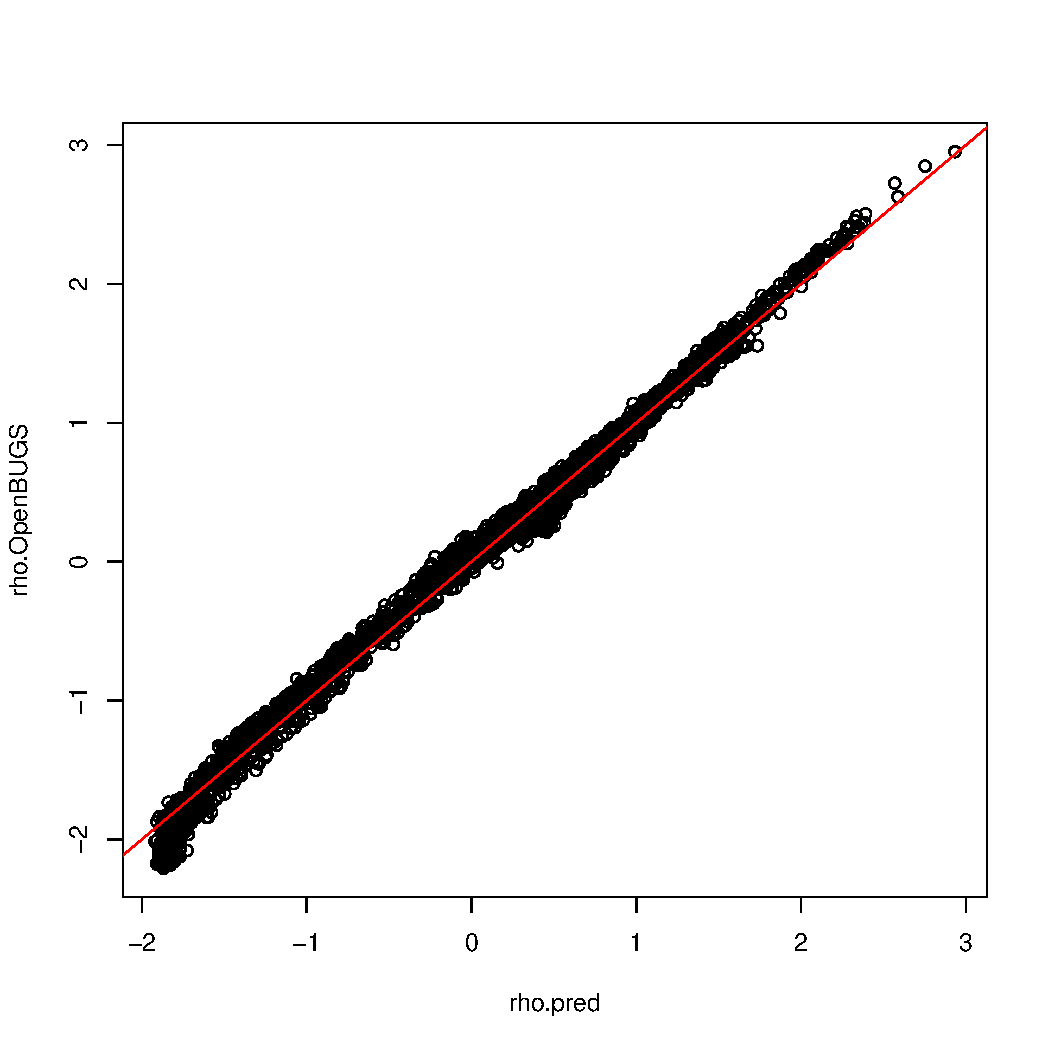
\includegraphics[width=8cm]{figures/binom-iCAR-openBUGS.pdf}
  \caption{\textbf{Comparison between hSDM and OpenBUGS for spatial random effect estimates.}}
  \label{fig:binom-iCAR-results}
\end{figure}

\newpage

\subsubsection{With a GLM}

\begin{knitrout}\small
\definecolor{shadecolor}{rgb}{0.969, 0.969, 0.969}\color{fgcolor}\begin{kframe}
\begin{alltt}
\hlcom{#== glm results for comparison}
\hlstd{mod.glm} \hlkwb{<-} \hlkwd{glm}\hlstd{(}\hlkwd{cbind}\hlstd{(Y,visits)}\hlopt{~}\hlstd{alt,}\hlkwc{family}\hlstd{=}\hlstr{"binomial"}\hlstd{,}\hlkwc{data}\hlstd{=data.suit)}
\hlkwd{summary}\hlstd{(mod.glm)}
\end{alltt}
\begin{verbatim}
## 
## Call:
## glm(formula = cbind(Y, visits) ~ alt, family = "binomial", data = data.suit)
## 
## Deviance Residuals: 
##    Min      1Q  Median      3Q     Max  
## -1.738  -0.883  -0.511   0.291   2.257  
## 
## Coefficients:
##             Estimate Std. Error z value Pr(>|z|)    
## (Intercept)  -1.2228     0.0924   -13.2  < 2e-16 ***
## alt           0.6302     0.1126     5.6  2.2e-08 ***
## ---
## Signif. codes:  0 '***' 0.001 '**' 0.01 '*' 0.05 '.' 0.1 ' ' 1
## 
## (Dispersion parameter for binomial family taken to be 1)
## 
##     Null deviance: 166.80  on 199  degrees of freedom
## Residual deviance: 127.05  on 198  degrees of freedom
## AIC: 339.9
## 
## Number of Fisher Scoring iterations: 4
\end{verbatim}
\end{kframe}
\end{knitrout}


\begin{knitrout}\small
\definecolor{shadecolor}{rgb}{0.969, 0.969, 0.969}\color{fgcolor}\begin{kframe}
\begin{alltt}
\hlcom{# Create a raster for predictions}
\hlstd{theta.pred.glm} \hlkwb{<-} \hlkwd{raster}\hlstd{(theta)}
\hlcom{# Attribute predicted values to raster cells}
\hlstd{theta.pred.glm[]} \hlkwb{<-} \hlkwd{predict.glm}\hlstd{(mod.glm,}\hlkwc{newdata}\hlstd{=data.pred,}\hlkwc{type}\hlstd{=}\hlstr{"response"}\hlstd{)}
\hlcom{# Plot the predicted probability of presence}
\hlkwd{plot}\hlstd{(theta.pred.glm,}\hlkwc{main}\hlstd{=}\hlstr{"GLM for iCAR"}\hlstd{,}\hlkwc{col}\hlstd{=}\hlkwd{colRP}\hlstd{(nb),}\hlkwc{breaks}\hlstd{=brks,}
     \hlkwc{axis.args}\hlstd{=arg,}\hlkwc{zlim}\hlstd{=}\hlkwd{c}\hlstd{(}\hlnum{0}\hlstd{,}\hlnum{1}\hlstd{))}
\end{alltt}
\end{kframe}
\end{knitrout}


\begin{knitrout}\small
\definecolor{shadecolor}{rgb}{0.969, 0.969, 0.969}\color{fgcolor}\begin{kframe}
\begin{alltt}
\hlcom{# Comparing predictions to initial values}
\hlkwd{plot}\hlstd{(theta[],theta.pred.glm[],}
     \hlkwc{xlim}\hlstd{=}\hlkwd{c}\hlstd{(}\hlnum{0}\hlstd{,}\hlnum{1}\hlstd{),}\hlkwc{ylim}\hlstd{=}\hlkwd{c}\hlstd{(}\hlnum{0}\hlstd{,}\hlnum{1}\hlstd{),}\hlkwc{cex.lab}\hlstd{=}\hlnum{1.4}\hlstd{)}
\hlkwd{abline}\hlstd{(}\hlkwc{a}\hlstd{=}\hlnum{0}\hlstd{,}\hlkwc{b}\hlstd{=}\hlnum{1}\hlstd{,}\hlkwc{col}\hlstd{=}\hlstr{"red"}\hlstd{,}\hlkwc{lwd}\hlstd{=}\hlnum{2}\hlstd{)}
\end{alltt}
\end{kframe}
\end{knitrout}


\begin{figure} 
  \begin{tabular}{cc}
    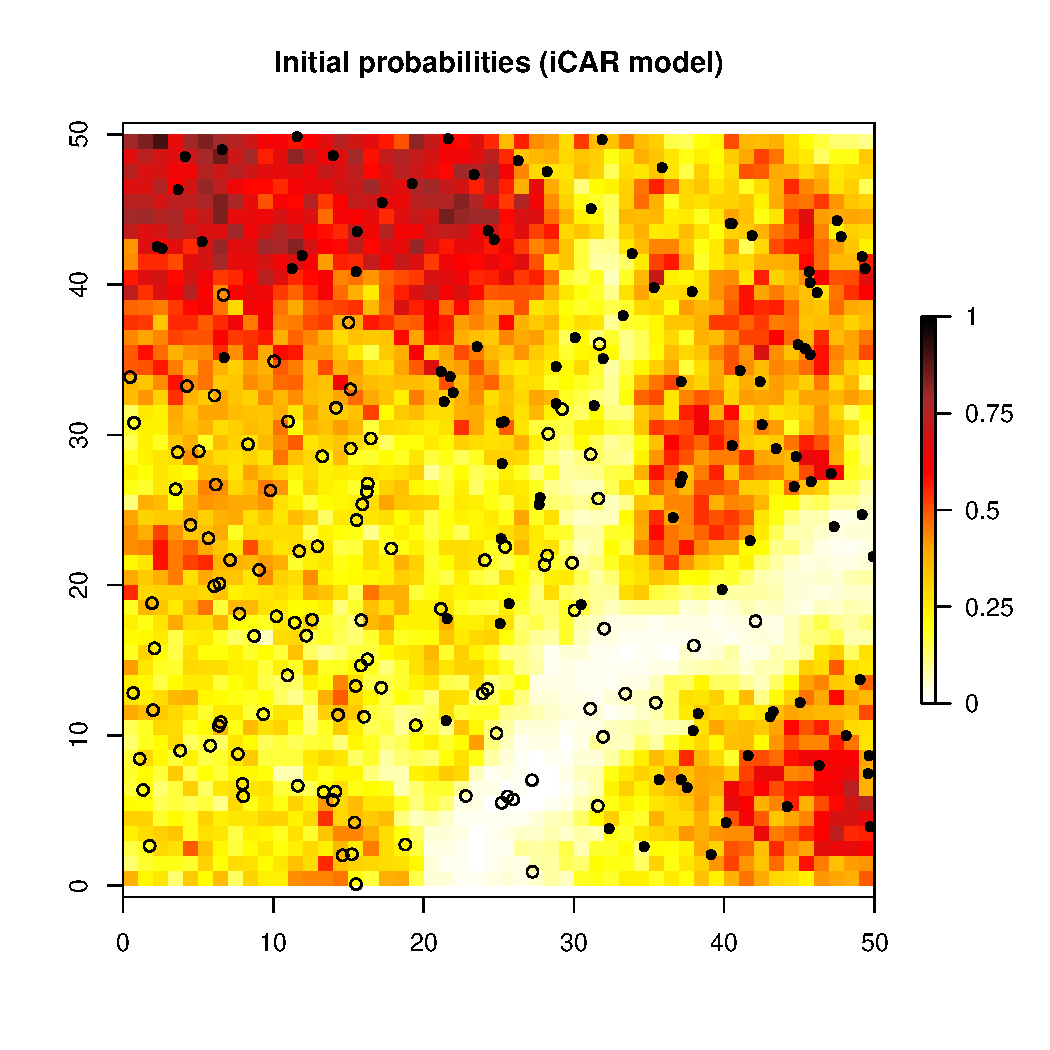
\includegraphics[width=6.5cm]{figures/binom-iCAR-plots2.pdf} &
    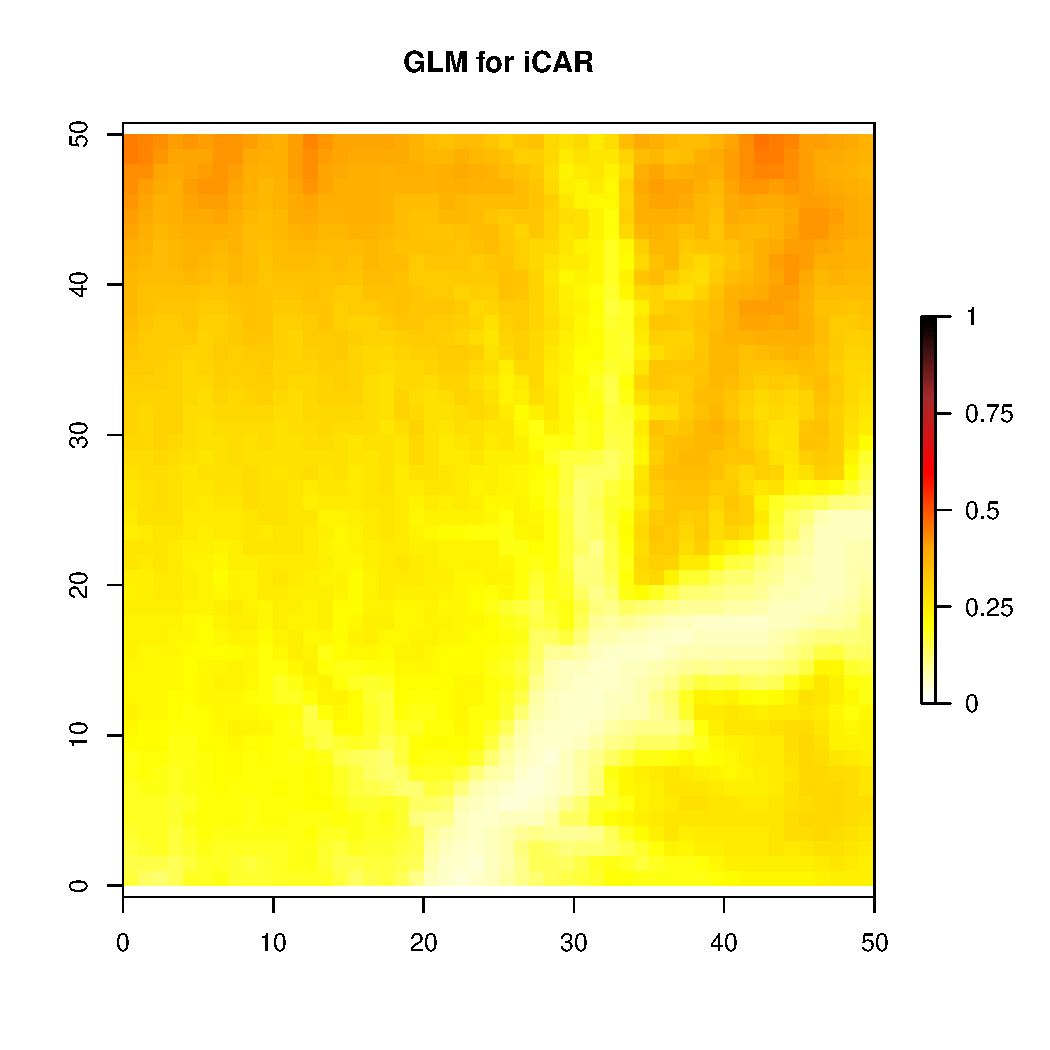
\includegraphics[width=6.5cm]{figures/predictions-binom-iCAR-glm.pdf} \\
  \end{tabular}
  \centering 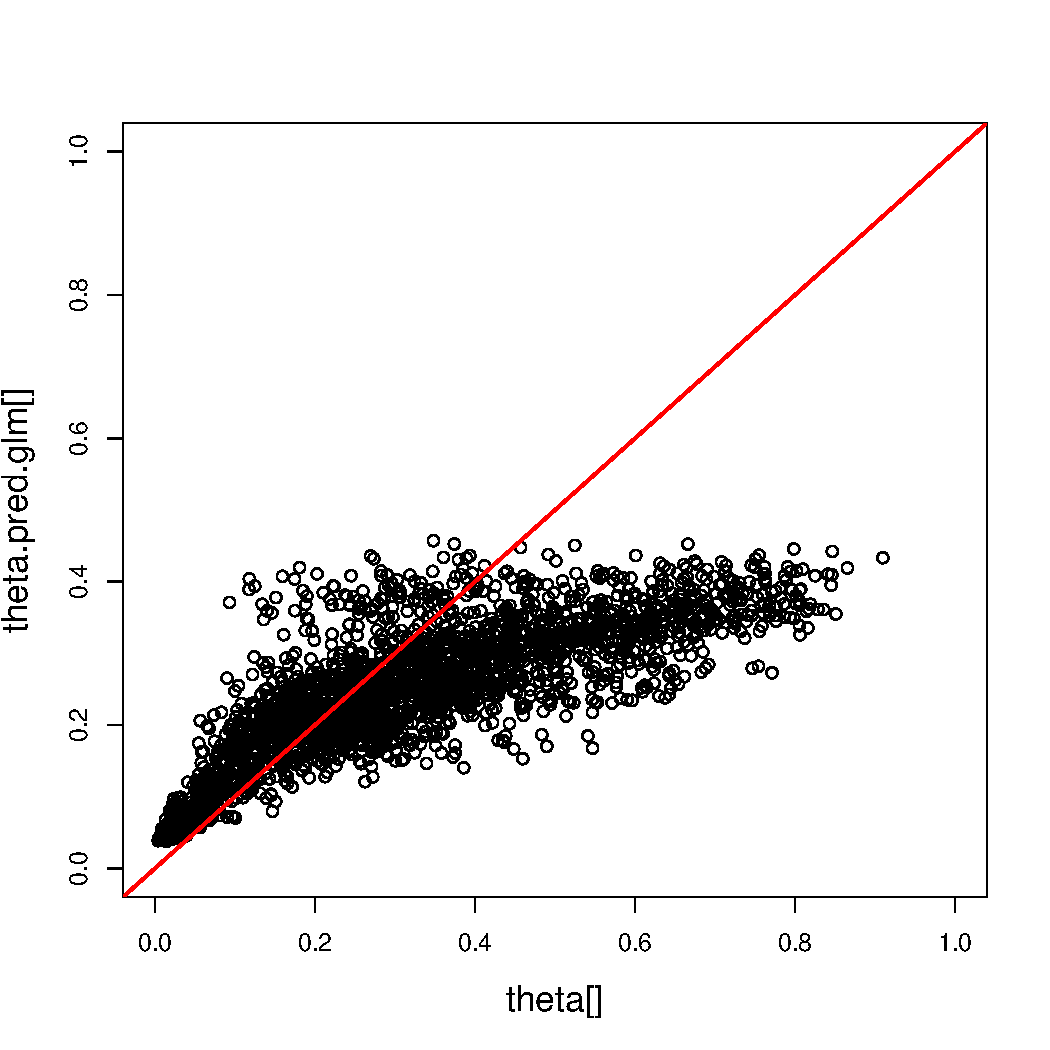
\includegraphics[width=8cm]{figures/pred-obs-binom-iCAR-glm.pdf} \\
  
  \caption{\textbf{Comparing predicted probability of presence using GLM with initial
      probabilities for a binomial model with iCAR process.}}
  
  \label{fig:predictions-siteocc-glm}
  
\end{figure}

\newpage

\subsection{Site-occupancy iCAR model}



\newpage

\section{Acknowledgements}

Support was provided by Cirad and FRB (Fondation pour la Recherche sur la Biodiversité)
through the BioSceneMada project (project agreement AAP-SCEN-2013 I).

\newpage

\bibliographystyle{gcb}
\bibliography{/home/ghislain/Documents/Ghislain-CIRAD/Biblio/Biblio-These-GV}

\end{document}
